% The manuscript; hh-dynamics.pdf beside it is this file built with pdflatex, run three times (sh tools/paper-build.sh
% hh-dynamics).  Every number that a program prints comes from the generated block below, which ../code/hh_make_numbers.py
% writes from ../data/*.txt; the figures are written by ../code/hh_make_figures.py.  Paths such as code/certlib.py are
% relative to the paper's folder (the folder that holds paper/, code/ and data/).
\documentclass[11pt]{article}
\usepackage[letterpaper,margin=1in]{geometry}
\usepackage[T1]{fontenc}
\usepackage{lmodern}
\usepackage{amsmath,amssymb,amsthm}
\usepackage{graphicx}
\usepackage{array}
\usepackage{booktabs}
\usepackage{microtype}
\setlength{\emergencystretch}{2em}
\usepackage[font=small,skip=4pt]{caption}
\usepackage[hidelinks]{hyperref}

\hypersetup{
  pdftitle={Hopf Bifurcations and Bistability in the Hodgkin-Huxley Equations at the 1952 Parameters: Computer-Assisted Proofs},
  pdfauthor={Chase Hendrick}}

\newtheorem{theorem}{Theorem}
\newtheorem{corollary}[theorem]{Corollary}
\newtheorem{lemma}{Lemma}[section]
\newtheorem{proposition}[lemma]{Proposition}
\newtheorem{citedtheorem}{Theorem}
% The two cited theorems are lettered: H (Andronov-Hopf) and K (Krawczyk), so that they are not confused with the
% numbered results of this paper.
\renewcommand{\thecitedtheorem}{\ifcase\value{citedtheorem}\or H\or K\fi}
\theoremstyle{definition}
\newtheorem{definition}[lemma]{Definition}
\newtheorem{remark}[lemma]{Remark}

\renewcommand{\topfraction}{0.9}
\renewcommand{\textfraction}{0.1}
\renewcommand{\floatpagefraction}{0.8}

\newcommand{\R}{\mathbb{R}}
\newcommand{\C}{\mathbb{C}}
\newcommand{\re}{\operatorname{Re}}
\newcommand{\im}{\operatorname{Im}}
\newcommand{\eps}{\varepsilon}
\newcommand{\Jss}{J_{\mathrm{ss}}}
\newcommand{\ELs}{E_l^*}
\newcommand{\hull}{\operatorname{hull}}
\newcommand{\inter}{\operatorname{int}}
\newcommand{\dist}{\operatorname{dist}}
\DeclareUrlCommand\file{\urlstyle{tt}}

% BEGIN generated by code/hh_make_numbers.py from the reports in data/; do not edit by hand.
% Intervals are rounded outward from the printed balls; rerun the programs, then python3 code/hh_make_numbers.py.
\newcommand{\BiChecks}{93}
\newcommand{\BiCkpt}{0}
\newcommand{\BiControls}{27}
\newcommand{\BiLedger}{334}
\newcommand{\BiNumerical}{7}
\newcommand{\BiOrder}{20}
\newcommand{\BiPrec}{96}
\newcommand{\BiProof}{36}
\newcommand{\BiSelftests}{23}
\newcommand{\BiStageOneNeg}{13}
\newcommand{\BiStageOneTests}{36}
\newcommand{\BiTimeFourB}{1707}
\newcommand{\BiTimeMin}{53.1}
\newcommand{\BiTimeNumerics}{886}
\newcommand{\BiTol}{1\cdot 10^{-18}}
\newcommand{\BiWorkers}{2}
\newcommand{\ClusterOne}{[5.345749617,\allowbreak 5.345961571]}
\newcommand{\ClusterTwo}{[21.941817522,\allowbreak 21.941999197]}
\newcommand{\CrossrelOne}{3.23\cdot 10^{-40}}
\newcommand{\CrossrelTwo}{6.24\cdot 10^{-41}}
\newcommand{\CtlKJ}{4.5\cdot 10^{10}}
\newcommand{\CtlKappaHi}{0.5439}
\newcommand{\CtlNorm}{37.997}
\newcommand{\CtlTwentyDthree}{[-18.86,\allowbreak -17.14]}
\newcommand{\CtlTwentyDtwo}{[-4.32,\allowbreak -3.68]}
\newcommand{\CtlTwentyU}{[8.405,\allowbreak 8.415]}
\newcommand{\ELstar}{[10.5989209693916785221988785,\allowbreak 10.5989209693916785221988786]}
\newcommand{\ELstarBiPrinted}{[10.5989209693916785221988785 \pm 6.21\cdot 10^{-26}]}
\newcommand{\ELstarCheck}{[10.5989209693916785221988785294,\allowbreak 10.5989209693916785221988785295]}
\newcommand{\ELstarShort}{10.5989209693916}
\newcommand{\EqAFour}{[0.1929,\allowbreak 0.2071]}
\newcommand{\EqAOne}{[4.8848,\allowbreak 4.8952]}
\newcommand{\EqAThree}{[1.5908,\allowbreak 1.6092]}
\newcommand{\EqATwo}{[1.2753,\allowbreak 1.3247]}
\newcommand{\EqBoxh}{[0.42941,\allowbreak 0.43059]}
\newcommand{\EqBoxm}{[0.0900353,\allowbreak 0.0901647]}
\newcommand{\EqBoxn}{[0.3905195,\allowbreak 0.3906805]}
\newcommand{\EqBoxu}{[4.64375,\allowbreak 4.65625]}
\newcommand{\EqDiscFour}{-0.135017}
\newcommand{\EqDiscImFour}{0.000000}
\newcommand{\EqDiscImOne}{0.000000}
\newcommand{\EqDiscImThree}{-0.566815}
\newcommand{\EqDiscImTwo}{0.566815}
\newcommand{\EqDiscOne}{-4.690211}
\newcommand{\EqDiscRFour}{6.1\cdot 10^{-5}}
\newcommand{\EqDiscROne}{6.9\cdot 10^{-3}}
\newcommand{\EqDiscRThree}{8.4\cdot 10^{-3}}
\newcommand{\EqDiscRTwo}{8.4\cdot 10^{-3}}
\newcommand{\EqDiscThree}{-0.034513}
\newcommand{\EqDiscTwo}{-0.034513}
\newcommand{\EqDthree}{[2.406,\allowbreak 3.594]}
\newcommand{\EqDtwo}{[4.616,\allowbreak 4.784]}
\newcommand{\EqExcl}{70}
\newcommand{\EqHighBound}{23.31}
\newcommand{\EqNewtonDF}{[2.3706,\allowbreak 2.4294]}
\newcommand{\EqNewtonN}{[4.64373,\allowbreak 4.65627]}
\newcommand{\EqNewtonU}{[4.64089,\allowbreak 4.65911]}
\newcommand{\EqW}{[3.646624,\allowbreak 5.646624]}
\newcommand{\EqWpieces}{64}
\newcommand{\ExtrapRatio}{34.65}
\newcommand{\FLINTVersion}{3.6.0}
\newcommand{\FlintVersion}{0.9.0}
\newcommand{\FoldFreq}{50.3}
\newcommand{\FoldHH}{6.260321}
\newcommand{\FoldPeriod}{19.8952}
\newcommand{\FoldStar}{6.264545}
\newcommand{\FreqHi}{62.478}
\newcommand{\FreqLo}{62.445}
\newcommand{\HopfChecks}{40}
\newcommand{\HopfConsistency}{6}
\newcommand{\HopfControls}{5}
\newcommand{\HopfCross}{4}
\newcommand{\HopfLedger}{99}
\newcommand{\HopfProof}{17}
\newcommand{\HopfSelftests}{8}
\newcommand{\HopfTime}{7}
\newcommand{\HopfVersions}{python-flint 0.9.0 on FLINT 3.6.0}
\newcommand{\HpSmu}{0.07089678069271872876}
\newcommand{\HpTs}{16.00771280383757999237802}
\newcommand{\HpTu}{14.34360094817270692874908}
\newcommand{\HpUmuOne}{10.3028828212211696095}
\newcommand{\HpUmuTwo}{0.19683222913631744833}
\newcommand{\HtwoDeltaA}{1}
\newcommand{\HtwoDeltaB}{0.5}
\newcommand{\HtwoDeltaC}{0.25}
\newcommand{\HtwoExtrap}{14.29}
\newcommand{\HtwoMuMax}{0.987}
\newcommand{\HtwoRatioA}{14.42}
\newcommand{\HtwoRatioB}{14.36}
\newcommand{\HtwoRatioC}{14.32}
\newcommand{\IdChecks}{33}
\newcommand{\IdControls}{6}
\newcommand{\IdCross}{8}
\newcommand{\IdCtlMin}{10}
\newcommand{\IdLedger}{12}
\newcommand{\IdOffMax}{0.18}
\newcommand{\IdPieces}{$[10.5985, 10.5990]$, $[10.5990, 10.5995]$, $[10.6125, 10.6130]$, $[10.6130, 10.6135]$}
\newcommand{\IdProof}{19}
\newcommand{\IdTime}{244}
\newcommand{\Irest}{[-0.004223709183,\allowbreak -0.004223709182]}
\newcommand{\IrestShort}{-0.004223}
\newcommand{\JHOneGO}{[9.779637995393,\allowbreak 9.779637995394]}
\newcommand{\JHOneGOlong}{[9.7796379953931263,\allowbreak 9.7796379953931264]}
\newcommand{\JHOneHH}{[9.775437995393,\allowbreak 9.775437995394]}
\newcommand{\JHOneHHlong}{[9.7754379953931263,\allowbreak 9.7754379953931264]}
\newcommand{\JHOneHi}{[9.773337995393,\allowbreak 9.773337995394]}
\newcommand{\JHOneHilong}{[9.7733379953931263,\allowbreak 9.7733379953931264]}
\newcommand{\JHOneLo}{[9.782337995393,\allowbreak 9.782337995394]}
\newcommand{\JHOneLolong}{[9.7823379953931263,\allowbreak 9.7823379953931264]}
\newcommand{\JHOneRange}{[9.773337995,\allowbreak 9.782337996]}
\newcommand{\JHOneStar}{[9.779661704575,\allowbreak 9.779661704576]}
\newcommand{\JHOneStarlong}{[9.7796617045756227,\allowbreak 9.7796617045756228]}
\newcommand{\JHTwoGO}{[154.526633665808,\allowbreak 154.526633665809]}
\newcommand{\JHTwoGOlong}{[154.5266336658080008,\allowbreak 154.5266336658080009]}
\newcommand{\JHTwoHH}{[154.522433665808,\allowbreak 154.522433665809]}
\newcommand{\JHTwoHHlong}{[154.5224336658080008,\allowbreak 154.5224336658080009]}
\newcommand{\JHTwoHi}{[154.520333665808,\allowbreak 154.520333665809]}
\newcommand{\JHTwoHilong}{[154.5203336658080008,\allowbreak 154.5203336658080009]}
\newcommand{\JHTwoLo}{[154.529333665808,\allowbreak 154.529333665809]}
\newcommand{\JHTwoLolong}{[154.5293336658080008,\allowbreak 154.5293336658080009]}
\newcommand{\JHTwoRange}{[154.520333665,\allowbreak 154.529333666]}
\newcommand{\JHTwoStar}{[154.526657374990,\allowbreak 154.526657374991]}
\newcommand{\JHTwoStarlong}{[154.5266573749904973,\allowbreak 154.5266573749904974]}
\newcommand{\JHoneMinBall}{9.773337}
\newcommand{\JequivHi}{8.0021}
\newcommand{\JequivLo}{7.9931}
\newcommand{\JssBoundHigh}{4089.4815}
\newcommand{\JssMinusTwelve}{-6.7999}
\newcommand{\MutByCheck}{16}
\newcommand{\MutByExc}{0}
\newcommand{\MutSign}{[-0.19019608,\allowbreak -0.19019607]}
\newcommand{\MutStopped}{16}
\newcommand{\MutStrong}{16}
\newcommand{\MutTime}{37}
\newcommand{\MutTotal}{17}
\newcommand{\MutTwoiw}{[2.9666666,\allowbreak 2.9666667]}
\newcommand{\MutWeak}{1}
\newcommand{\MutWeakPassed}{1}
\newcommand{\NPieces}{60}
\newcommand{\NormMax}{0.5446}
\newcommand{\NormMin}{0.5413}
\newcommand{\Normball}{0.5446}
\newcommand{\NpiecesHurwitz}{1043}
\newcommand{\NpiecesSlope}{74}
\newcommand{\NumDeltaU}{3.806769951380}
\newcommand{\NumIssTwoFifty}{9418.0}
\newcommand{\NumRest}{3.620669\cdot 10^{-3}}
\newcommand{\NumSumax}{95.9574}
\newcommand{\NumTs}{16.007712803838}
\newcommand{\Nundecided}{52}
\newcommand{\PerOne}{[10.717882807,\allowbreak 10.717882808]}
\newcommand{\PerTwo}{[5.911239441,\allowbreak 5.911239442]}
\newcommand{\PieceBoxRad}{4.6\cdot 10^{-7}}
\newcommand{\PieceTimeMax}{77}
\newcommand{\PieceTimeMin}{37}
\newcommand{\PieceWidth}{5\cdot 10^{-4}}
\newcommand{\PythonVersion}{3.11.15}
\newcommand{\SDPradGO}{1.11\cdot 10^{-9}}
\newcommand{\SDPradHH}{1.10\cdot 10^{-9}}
\newcommand{\SDPradStar}{1.11\cdot 10^{-9}}
\newcommand{\SboxRadGO}{1.22\cdot 10^{-15}}
\newcommand{\SboxRadHH}{1.21\cdot 10^{-15}}
\newcommand{\SboxRadStar}{1.22\cdot 10^{-15}}
\newcommand{\SlopeOne}{[34.657379,\allowbreak 34.657380]}
\newcommand{\SlopeShortOne}{34.65}
\newcommand{\SlopeShortTwo}{14.29}
\newcommand{\SlopeTwo}{[14.292859,\allowbreak 14.292860]}
\newcommand{\SmaxLoGO}{95.953706}
\newcommand{\SmaxLoHH}{95.953532}
\newcommand{\SmaxLoStar}{95.953707}
\newcommand{\SminHiGO}{-10.140154}
\newcommand{\SminHiHH}{-10.139662}
\newcommand{\SminHiStar}{-10.140157}
\newcommand{\SmuOneGO}{0.070904221789}
\newcommand{\SmuOneHH}{0.070896780693}
\newcommand{\SmuOneRGO}{2.26\cdot 10^{-9}}
\newcommand{\SmuOneRHH}{2.25\cdot 10^{-9}}
\newcommand{\SmuOneRStar}{2.26\cdot 10^{-9}}
\newcommand{\SmuOneStar}{0.070904264160}
\newcommand{\SmuRestGO}{3.99\cdot 10^{-9}}
\newcommand{\SmuRestHH}{3.97\cdot 10^{-9}}
\newcommand{\SmuRestStar}{3.99\cdot 10^{-9}}
\newcommand{\SpassesGO}{1}
\newcommand{\SpassesHH}{1}
\newcommand{\SpassesStar}{1}
\newcommand{\SplitControl}{[-0.0004982,\allowbreak -0.0004981]}
\newcommand{\SpthGO}{[0.39231447350,\allowbreak 0.39231447351]}
\newcommand{\SpthHH}{[0.39231037641,\allowbreak 0.39231037642]}
\newcommand{\SpthStar}{[0.39231449643,\allowbreak 0.39231449644]}
\newcommand{\SptmGO}{[0.24053255147,\allowbreak 0.24053255148]}
\newcommand{\SptmHH}{[0.24052906069,\allowbreak 0.24052906070]}
\newcommand{\SptmStar}{[0.24053257124,\allowbreak 0.24053257125]}
\newcommand{\SptnGO}{[0.42490308639,\allowbreak 0.42490308640]}
\newcommand{\SptnHH}{[0.42490470823,\allowbreak 0.42490470824]}
\newcommand{\SptnStar}{[0.42490307734,\allowbreak 0.42490307735]}
\newcommand{\SrangeGO}{[-10.155224,\allowbreak 96.045294]}
\newcommand{\SrangeHH}{[-10.154729,\allowbreak 96.045119]}
\newcommand{\SrangeStar}{[-10.155227,\allowbreak 96.045295]}
\newcommand{\SstepsGO}{303}
\newcommand{\SstepsHH}{303}
\newcommand{\SstepsStar}{303}
\newcommand{\TballHi}{16.013912063}
\newcommand{\TballHiShort}{16.0140}
\newcommand{\TballLo}{16.005827509}
\newcommand{\TballLoShort}{16.0058}
\newcommand{\TestCoupledA}{[0.143137254901,\allowbreak 0.143137254902]}
\newcommand{\TestCoupledB}{[-0.101501501502,\allowbreak -0.101501501501]}
\newcommand{\TestPlanarA}{[-0.160416666667,\allowbreak -0.160416666666]}
\newcommand{\TestPlanarB}{[0.125573192239,\allowbreak 0.125573192240]}
\newcommand{\TransrelOne}{5.9\cdot 10^{-27}}
\newcommand{\TransrelTwo}{2.7\cdot 10^{-27}}
\newcommand{\TsGO}{[16.01148299894,\allowbreak 16.01148299895]}
\newcommand{\TsHH}{[16.00771280383,\allowbreak 16.00771280384]}
\newcommand{\TsStar}{[16.01150429806,\allowbreak 16.01150429807]}
\newcommand{\TuGO}{[14.36930333,\allowbreak 14.36930334]}
\newcommand{\TuHH}{[14.34360094,\allowbreak 14.34360095]}
\newcommand{\TuStar}{[14.36944974,\allowbreak 14.36944975]}
\newcommand{\UDPradGO}{1.56\cdot 10^{-4}}
\newcommand{\UDPradHH}{1.29\cdot 10^{-4}}
\newcommand{\UDPradStar}{7.90\cdot 10^{-5}}
\newcommand{\UballMax}{95.953}
\newcommand{\UboxRadGO}{2.13\cdot 10^{-14}}
\newcommand{\UboxRadHH}{2.13\cdot 10^{-14}}
\newcommand{\UboxRadMinGO}{1.94\cdot 10^{-15}}
\newcommand{\UboxRadMinHH}{2.03\cdot 10^{-15}}
\newcommand{\UboxRadMinStar}{1.00\cdot 10^{-15}}
\newcommand{\UboxRadStar}{1.08\cdot 10^{-14}}
\newcommand{\UmaxHiGO}{11.073666}
\newcommand{\UmaxHiHH}{11.045813}
\newcommand{\UmaxHiStar}{11.073821}
\newcommand{\UmuOneGO}{[10.52836245,\allowbreak 10.52886553]}
\newcommand{\UmuOneHH}{[10.30268246,\allowbreak 10.30308318]}
\newcommand{\UmuOneStar}{[10.52978728,\allowbreak 10.53004150]}
\newcommand{\UmuThreeGO}{1.88\cdot 10^{-4}}
\newcommand{\UmuThreeHH}{1.57\cdot 10^{-4}}
\newcommand{\UmuThreeStar}{9.49\cdot 10^{-5}}
\newcommand{\UmuTwoGO}{0.1971736153}
\newcommand{\UmuTwoHH}{0.1968322291}
\newcommand{\UmuTwoRGO}{3.51\cdot 10^{-4}}
\newcommand{\UmuTwoRHH}{2.72\cdot 10^{-4}}
\newcommand{\UmuTwoRStar}{1.78\cdot 10^{-4}}
\newcommand{\UmuTwoStar}{0.1971756106}
\newcommand{\UpassesGO}{1}
\newcommand{\UpassesHH}{1}
\newcommand{\UpassesStar}{1}
\newcommand{\UpthGO}{[0.43755917467,\allowbreak 0.43755917468]}
\newcommand{\UpthHH}{[0.43754826309,\allowbreak 0.43754826310]}
\newcommand{\UpthStar}{[0.43755923369,\allowbreak 0.43755923370]}
\newcommand{\UptmGO}{[0.09003972849,\allowbreak 0.09003972850]}
\newcommand{\UptmHH}{[0.09004142752,\allowbreak 0.09004142753]}
\newcommand{\UptmStar}{[0.09003971888,\allowbreak 0.09003971889]}
\newcommand{\UptnGO}{[0.37946696511,\allowbreak 0.37946696512]}
\newcommand{\UptnHH}{[0.37950318996,\allowbreak 0.37950318997]}
\newcommand{\UptnStar}{[0.37946676035,\allowbreak 0.37946676036]}
\newcommand{\UrangeGO}{[-0.728092,\allowbreak 11.073666]}
\newcommand{\UrangeHH}{[-0.709090,\allowbreak 11.045813]}
\newcommand{\UrangeStar}{[-0.728187,\allowbreak 11.073821]}
\newcommand{\UstepsGO}{112}
\newcommand{\UstepsHH}{112}
\newcommand{\UstepsStar}{112}
\newcommand{\dDthreeOne}{[-4.121,\allowbreak -4.109]}
\newcommand{\dDthreeTwo}{[176.1,\allowbreak 176.6]}
\newcommand{\dJuOne}{[2.67128168,\allowbreak 2.67128169]}
\newcommand{\dJuTwo}{[18.34451285,\allowbreak 18.34451286]}
\newcommand{\dlJOne}{[0.01878905889,\allowbreak 0.01878905890]}
\newcommand{\dlJTwo}{[-0.00449227917,\allowbreak -0.00449227916]}
\newcommand{\dluOne}{[0.0501908689,\allowbreak 0.0501908690]}
\newcommand{\dluTwo}{[-0.0824086729,\allowbreak -0.0824086728]}
\newcommand{\dzdE}{-0.000249}
\newcommand{\loneOne}{[0.01479364813100,\allowbreak 0.01479364813101]}
\newcommand{\loneTwo}{[-0.004728502695074,\allowbreak -0.004728502695073]}
\newcommand{\omOne}{[0.586233813130,\allowbreak 0.586233813131]}
\newcommand{\omTwo}{[1.062921806760,\allowbreak 1.062921806761]}
\newcommand{\quOne}{[0.9999042898,\allowbreak 0.9999042899]}
\newcommand{\quTwo}{[0.9997206845,\allowbreak 0.9997206846]}
\newcommand{\uHOne}{[5.345856397004594535603253257542,\allowbreak 5.345856397004594535603253257543]}
\newcommand{\uHOnerad}{2.28\cdot 10^{-73}}
\newcommand{\uHOneshort}{[5.345856397004,\allowbreak 5.345856397005]}
\newcommand{\uHTwo}{[21.941907987016173702380109736212,\allowbreak 21.941907987016173702380109736213]}
\newcommand{\uHTworad}{3.69\cdot 10^{-73}}
\newcommand{\uHTwoshort}{[21.941907987016,\allowbreak 21.941907987017]}
\newcommand{\uStarGO}{[4.644881448682,\allowbreak 4.644881448683]}
\newcommand{\uStarHH}{[4.646624016873,\allowbreak 4.646624016874]}
\newcommand{\uStarStar}{[4.644871610529,\allowbreak 4.644871610530]}
\newcommand{\TabBranchRows}{%
8.50 & 12.6126 & 8.1128 & 1.2754 & 51.60 \\
9.00 & 11.6921 & 5.7233 & 0.7754 & 42.24 \\
9.50 & 11.0248 & 3.1849 & 0.2754 & 36.83 \\
9.70 & 10.7986 & 1.6298 & 0.0754 & 35.21 \\
9.75 & 10.7448 & 0.9414 & 0.0254 & 34.84 \\}
\newcommand{\TabFilesRows}{%
\texttt{code/certify\_equilibria\_hopf.py} & \texttt{c2592f1e4559a8d4} \\
\texttt{code/hh\_ball.py} & \texttt{754623075e174f8d} \\
\texttt{code/certify\_bistability.py} & \texttt{49a0da01e7a03c56} \\
\texttt{code/hh\_arb.py} & \texttt{88321fe660c541fd} \\
\texttt{code/hh\_lohner.py} & \texttt{7dd88ec6057acff6} \\
\texttt{code/certlib.py} & \texttt{aab30999170cc70c} \\
\texttt{code/ball\_stable.py} & \texttt{a7acfc9e5a168c49} \\
\texttt{code/outward.py} & \texttt{417e163289459752} \\
\texttt{code/tests\_integrator.py} & \texttt{6e8417d0b6bff303} \\
\texttt{code/testsys.py} & \texttt{bbb47b4132b0164e} \\
\texttt{code/shoot\_float.py} & \texttt{077dbbb104ba0f7f} \\
\texttt{code/hh\_numerics.py} & \texttt{f48dc49e46fca474} \\
\texttt{code/identify\_stable\_orbit.py} & \texttt{83564add9d2465b4} \\
\texttt{code/mutation\_study.py} & \texttt{782f5b11f93770cd} \\
\texttt{data/certify\_equilibria\_hopf.txt} & \texttt{add0ef88d9f2306f} \\
\texttt{data/certify\_bistability.txt} & \texttt{62908b21151b309f} \\
\texttt{data/identify\_stable\_orbit.txt} & \texttt{3cc8546e0a84f4e9} \\
\texttt{data/mutation\_study.txt} & \texttt{d472c4d9e775d01d} \\}
\newcommand{\TabStableRows}{%
$10.613$ & $[16.00771280383, 16.00771280384]$ & $|\mu_1 - 0.070896780693| \le 2.25\cdot 10^{-9}$ & $3.97\cdot 10^{-9}$ \\
$E_l^*$ & $[16.01150429806, 16.01150429807]$ & $|\mu_1 - 0.070904264160| \le 2.26\cdot 10^{-9}$ & $3.99\cdot 10^{-9}$ \\
$10.599$ & $[16.01148299894, 16.01148299895]$ & $|\mu_1 - 0.070904221789| \le 2.26\cdot 10^{-9}$ & $3.99\cdot 10^{-9}$ \\}
\newcommand{\TabUnstableRows}{%
$10.613$ & $[14.34360094, 14.34360095]$ & $[10.30268246, 10.30308318]$ & $|\mu_2 - 0.1968322291| \le 2.72\cdot 10^{-4}$ & $1.57\cdot 10^{-4}$ \\
$E_l^*$ & $[14.36944974, 14.36944975]$ & $[10.52978728, 10.53004150]$ & $|\mu_2 - 0.1971756106| \le 1.78\cdot 10^{-4}$ & $9.49\cdot 10^{-5}$ \\
$10.599$ & $[14.36930333, 14.36930334]$ & $[10.52836245, 10.52886553]$ & $|\mu_2 - 0.1971736153| \le 3.51\cdot 10^{-4}$ & $1.88\cdot 10^{-4}$ \\}
% END generated by code/hh_make_numbers.py

\title{\Large\bfseries Hopf Bifurcations and Bistability in the Hodgkin-Huxley Equations\\ at the 1952 Parameters: Computer-Assisted Proofs}
\author{Chase Hendrick\\[0.2em] {\small Independent Researcher}\\ {\small\href{mailto:chase@hendrickresearch.com}{\texttt{chase@hendrickresearch.com}}}\\ {\small ORCID \href{https://orcid.org/0009-0002-9754-6087}{0009-0002-9754-6087}}}
\date{}

\begin{document}
\maketitle

\begin{abstract}
The space-clamped Hodgkin--Huxley equations with Hodgkin and Huxley's constants are the standard model of the action potential, and their bifurcations are known from numerical computation. We prove several of them with computer assistance in ball arithmetic, for every leak reversal potential $E_l$ in $[10.59, 10.62]$~mV, an interval that contains the value $10.613$ printed by Hodgkin and Huxley and the value $\ELs = \ELstarShort\ldots$ that makes the resting current zero, as their Table~3 says it should. For every applied current $J$ in $[0, 200]$~$\mu$A/cm$^2$ there is exactly one equilibrium. There are two Hopf points $J_{H1} < J_{H2}$ in this range: the equilibrium is asymptotically stable for $J < J_{H1}$ and for $J > J_{H2}$, it has exactly two eigenvalues with positive real part for $J_{H1} < J < J_{H2}$, and no eigenvalue lies on the imaginary axis at any current of the range other than $J_{H1}$ and $J_{H2}$. At $E_l = 10.613$ the Hopf points lie at $J_{H1} \in \JHOneHH$ and $J_{H2} \in \JHTwoHH$, and both move by exactly $0.3\,(10.613 - E_l)$ when $E_l$ changes. The eigenvalues cross the imaginary axis transversally, and the first Lyapunov coefficient is positive at $J_{H1}$ and negative at $J_{H2}$: the lower Hopf bifurcation is subcritical and the upper one supercritical. At $J = 8$, for every $E_l$ in the interval, a locally asymptotically stable equilibrium coexists with an orbitally asymptotically stable periodic orbit, a train of action potentials with period between $\TballLoShort$ and $\TballHiShort$~ms: the model is bistable there. At three values of $E_l$ we also enclose a periodic orbit of saddle type. The proofs combine a Routh--Hurwitz analysis along the branch of equilibria with a $C^1$ Lohner-type Taylor integrator, the Krawczyk test and a contraction argument on Poincar\'e sections. Nothing is claimed about the basins of attraction or about other attractors.

\medskip
\noindent\textbf{Keywords:} Hodgkin--Huxley equations; Hopf bifurcation; first Lyapunov coefficient; bistability; periodic orbit; computer-assisted proof; ball arithmetic.\\
\textbf{MSC 2020:} 92C20, 34C23, 37G15, 37C27, 65G20.
\end{abstract}

\section{Introduction}\label{sec:intro}

Hodgkin and Huxley's equations for the squid giant axon \cite{hh1952} are the prototype of a conductance-based neuron model. With the membrane potential uniform in space (the space clamp), they form a system of four ordinary differential equations in the depolarization $u$ and three gating variables $m$, $n$, $h$, with an applied current $J$ as the natural parameter. The picture of their dynamics that textbooks and later models rely on is numerical: a single equilibrium, stable for small and large currents and unstable in between; a Hopf bifurcation at each end of the unstable range, subcritical at the lower end near $J \approx 9.78$~$\mu$A/cm$^2$; and, below that current, a range in which the resting state coexists with repetitive firing, so that a brief pulse can start or stop a train of action potentials. Lu, Xin and Rinzel \cite[pp.~61--62]{lxr2023} review how the coexistence was found in simulations (they credit Cooley, Dodge and Cohen) and observed in the squid axon by Guttman, Lewis and Rinzel \cite{glr1980}; Best \cite{best1979} showed numerically that a suitable brief pulse stops the firing for good. This paper proves parts of that picture at Hodgkin and Huxley's own constants.

\paragraph{What is known.} The bifurcations of the space-clamped equations have been computed numerically many times; we cite only what we have read, and Section~\ref{sec:limits} says how far. Troy proved a Hopf bifurcation for a modified system in which $n$ and $h$ are slowed by a small parameter, under assumptions that he describes as ``made on the basis of numerical evidence and physical reasoning'' \cite[p.~76]{troy1978}, and large-amplitude periodic solutions for a reduced system of three equations under assumptions \cite{troy1977}; his earlier paper \cite{troy1976} proves Hopf bifurcation ``under appropriate assumptions'' (abstract). None of these is a proof for the full system at the 1952 constants. Hastings writes that the parameters ``appear, on the basis of numerical calculations, to be such that the system (3)--(4) has a unique equilibrium point'' \cite[p.~230]{hastings1976}; his system (3)--(4) is the traveling-wave system, whose equilibria are those of the space-clamped system at zero applied current. Guckenheimer and Labouriau state that when the potassium reversal potential has Hodgkin and Huxley's value, ``$f$ is monotonic and HH has a unique equilibrium for each value of $I$'' \cite[p.~941]{gl1993}, $f$ being the steady-state current (the same sentence is on p.~23 of the arXiv preprint of \cite{gw1993}); they give no proof, their computations of equilibria and of local bifurcations are symbolic (Macsyma, Mathematica and Maple) and their global ones numerical, and they write that their bifurcation diagrams in the plane of the current and the potassium reversal potential ``are conjectured on the basis of symbolic calculations, numerical computations and visual examination of a large number of phase portraits'' \cite[p.~938]{gl1993} and ``have not been proved to be correct'' \cite[p.~942]{gl1993}. Labouriau showed with singularity theory that the two branches of periodic solutions born at the Hopf points join, for the equations perturbed in parameters such as the temperature, and computed the invariants of the degenerate Hopf bifurcation that organizes them, which give a topological description of the periodic orbits near the equilibrium \cite{lab1985,lab1989}. Her thesis \cite{lab1983}, whose Chapter~IV (``Nerve impulse equations'') we have read, computes the eigenvalues along the branch of equilibria, the two Hopf points and the direction of bifurcation in floating point, with $V_L = 10.599$, and takes the invertibility of the steady-state current from a graph: ``within physiologically meaningful range $f$ is monotonically increasing (Fig.~IV-0-1)''; it states that ``all the information we have about HH, after reduction, is a numerical estimate of its derivatives''. Hassard and Shiau computed isolated branches of periodic solutions near degenerate Hopf points, with the temperature and the sodium conductance or reversal potential varied, by ``purely numerical techniques'' for the global branches \cite{hs1989,sh1991}, and computed, in the same way, a curve of doubly degenerate Hopf points in the parameters $(I, T, g_{\mathrm{Na}}, v_{\mathrm{Na}})$ with a special point of $Z_2$-codimension three, adding that ``we have not solved the unfolding problem'' \cite[p.~33]{hs1996}. Of \cite{lab1985,lab1989,hs1989,sh1991} we have read the abstracts, and \cite{hs1996} in full. Fukai, Doi, Nomura and Sato computed the bistable periodic solutions in several parameters \cite{fdns2000,fnds2000}. Guckenheimer and Oliva continued the periodic orbits born at the subcritical Hopf point and found chaotic dynamics near $J = 7.86$, adding that ``we do not give a rigorous proof that chaos exists in this system'' \cite[p.~106]{go2002}. The papers cited above also report the numerical Hopf computations of Hassard \cite{hassard1978} and the stable and unstable periodic solutions of Rinzel and Miller \cite{rm1980}. Du and Hassard \cite{dh2001} describe ``an algorithm \ldots\ for the computation of Hopf bifurcation coefficients for autonomous ordinary differential systems, by Lyapunov--Schmidt reduction'', in which ``interval values for the coefficients are found and it is known with mathematical certainty that the exact values fall in the computed intervals'', to solve the location and recognition problems of degenerate Hopf points of $Z_2$-codimension at most three, with ``applications to an enzyme-catalyzed reaction model and to the Hodgkin--Huxley nerve conduction model'' (abstract); the review in zbMATH adds that nondegeneracy conditions and the genericity of the unfolding are checked. Their method is local, concerned with the equilibrium and the periodic solutions near a Hopf point, and interval enclosures of the Hopf points of the model and of their coefficients may already be found there; we claim no priority for them. Computer-assisted proofs exist for the traveling pulse of the FitzHugh--Nagumo equations \cite{ak2015}, for their periodic traveling waves \cite{cz2016}, and for Hopf bubbles and degenerate Hopf bifurcations \cite{cq2024}; validated continuation of periodic orbits from a Hopf bifurcation is a general method \cite{blq2021}.

\paragraph{This paper.} We prove, for every leak reversal potential $E_l \in [10.59, 10.62]$:
\begin{itemize}
\item Theorem~\ref{thm:eq}: for every $J \in [0, 200]$ there is exactly one equilibrium.
\item Theorem~\ref{thm:hopf}: there are two currents $J_{H1} < J_{H2}$ such that along this branch the equilibrium is asymptotically stable for $J < J_{H1}$ and for $J > J_{H2}$, and has exactly two eigenvalues in $\re\lambda > 0$ for $J_{H1} < J < J_{H2}$; at $J_{Hi}$ it has a simple pair $\pm i\omega_i$ that crosses the imaginary axis transversally, and the first Lyapunov coefficient $\ell_1$ is positive at $J_{H1}$ and negative at $J_{H2}$. The currents are enclosed to $10^{-12}$.
\item Corollary~\ref{cor:hopf}: the Hopf bifurcation at $J_{H1}$ is subcritical and the one at $J_{H2}$ supercritical, in the sense of the normal form.
\item Theorem~\ref{thm:ball}: at $J = 8$ there is an orbitally asymptotically stable periodic orbit, a spike train with period in $[\TballLo, \TballHi]$~ms.
\item Theorem~\ref{thm:three}: at $J = 8$ and $E_l = 10.613$, $\ELs$ and $10.599$, a stable and a saddle-type periodic orbit, with narrow enclosures of their periods and Floquet multipliers; the stable one is the orbit of Theorem~\ref{thm:ball} (Corollary~\ref{cor:ident}).
\item Corollary~\ref{cor:bist}: bistability of rest and repetitive firing at $J = 8$, equivalently for $E_l = 10.613$ and every $J \in [\JequivLo, \JequivHi]$.
\end{itemize}
We have not found an earlier proof that the space-clamped Hodgkin--Huxley equations at the 1952 constants have a stable periodic orbit of large amplitude away from the Hopf points, such as the spike train of Theorem~\ref{thm:ball}, or that rest and repetitive firing are bistable. We claim no priority for Theorems~\ref{thm:eq} and~\ref{thm:hopf} or Corollary~\ref{cor:hopf}: Guckenheimer and Labouriau state the uniqueness of the equilibrium without proof, Du and Hassard's interval computations may already prove statements about the branch of equilibria, locate the Hopf points and fix their criticality, and a proved $\ell_1 < 0$ at $J_{H2}$ gives, with the Hopf theorem, the small stable cycles of Corollary~\ref{cor:hopf}(b). Du and Hassard describe a local method, the periodic solutions near a Hopf point, and neither their abstract nor the review in zbMATH mentions a periodic orbit away from the Hopf points or bistability. These statements are limited by the searches behind them, which Section~\ref{sec:limits} lists with the dates, or the range of dates, on which they were made, and how far each relevant paper was read.

\paragraph{Labels.} Every result carries a label. \emph{Proved}: a written proof in this paper, with no computation. \emph{Computer-assisted}: a written proof in which finitely many inequalities are decided by a program in ball arithmetic (Section~\ref{sec:method}); the program and the lines of its output that carry each step are named. \emph{Cited}: a published theorem used as stated in its source, with its hypotheses checked here; the two cited theorems are lettered, Theorems~\ref{thm:kuz} and~\ref{thm:krawczyk}. A result whose proof is computer-assisted and also uses a cited theorem says so in its label. \emph{Numerical}: floating-point or high-precision computation without error control; numerical results are never used in a proof and are collected in Section~\ref{sec:numerics}. Paths such as \file{code/certlib.py} name files of the folder that accompanies this paper. Section~\ref{sec:reproduce} says how to rerun everything, and Section~\ref{sec:limits} lists what is not proved and which checks of this work have been made.

\section{The model}\label{sec:model}

\subsection{The equations}

We use the modern sign convention: $u = -V$ is the depolarization from rest in mV, where $V$ is the displacement of Hodgkin and Huxley, and $J = -I$ is the applied depolarizing current in $\mu$A/cm$^2$; time is in ms and the temperature is $6.3^\circ$C, so no temperature factor enters. With the rate constants of \cite[eqs.~(12), (13), (20), (21), (23), (24)]{hh1952}, the current equation \cite[eq.~(26)]{hh1952} and the constants of \cite[Table~3]{hh1952} (the membrane capacity is $1~\mu$F/cm$^2$), the space-clamped equations read
\begin{equation}\label{eq:hh}
\begin{aligned}
  \dot u &= J - I(u, m, n, h), \qquad I = g_{\mathrm{Na}}\, m^3 h\, (u - E_{\mathrm{Na}}) + g_{\mathrm{K}}\, n^4 (u - E_{\mathrm{K}}) + g_l\, (u - E_l),\\
  \dot y &= \alpha_y(u)(1 - y) - \beta_y(u)\, y, \qquad y \in \{m, n, h\},
\end{aligned}
\end{equation}
with $g_{\mathrm{Na}} = 120$, $g_{\mathrm{K}} = 36$, $g_l = 0.3$, $E_{\mathrm{Na}} = 115$, $E_{\mathrm{K}} = -12$ and
\begin{equation}\label{eq:rates}
\begin{aligned}
  \alpha_m &= \Psi\bigl(\tfrac{25 - u}{10}\bigr), & \beta_m &= 4 e^{-u/18}, &
  \alpha_n &= 0.1\, \Psi\bigl(\tfrac{10 - u}{10}\bigr), & \beta_n &= 0.125\, e^{-u/80},\\
  \alpha_h &= 0.07\, e^{-u/20}, & \beta_h &= \frac{1}{e^{(30 - u)/10} + 1}, &
  \Psi(x) &= \frac{x}{e^x - 1},\ \Psi(0) = 1. &&
\end{aligned}
\end{equation}
We write $x = (u, m, n, h)$, $f(x; J, E_l)$ for the right-hand side of \eqref{eq:hh}, $k_y = \alpha_y + \beta_y$ and $y_\infty = \alpha_y/k_y$. Table~3 of \cite{hh1952} prints the leak potential $V_l = -10.613$~mV, that is $E_l = 10.613$, with the footnote ``Exact value chosen to make the total ionic current zero at the resting potential ($V = 0$)''.

\begin{lemma}[proved]\label{lem:basic}
(a) $\Psi(x) > 0$ and $\Psi'(x) < 0$ for every real $x$, so the six rates are positive and $y_\infty(u) \in (0, 1)$ for every $u \in \R$.
(b) $n_\infty$ is strictly increasing on $\R$.
(c) $f$ is real-analytic on $\R^4 \times \R^2$ (in $x$, $J$ and $E_l$).
(d) The equilibria of \eqref{eq:hh} are exactly the points $x^*(u) = (u, m_\infty(u), n_\infty(u), h_\infty(u))$ with $\Jss(u) = J$, where $\Jss(u) = I(x^*(u))$ is the steady-state current.
\end{lemma}

\begin{proof}
(a) $x$ and $e^x - 1$ have the same sign, so $\Psi > 0$. $\Psi'(x) = g(x)/(e^x - 1)^2$ with $g(x) = e^x - 1 - xe^x$ for $x \ne 0$; $g(0) = 0$ and $g'(x) = -xe^x$, so $g < 0$ for $x \ne 0$, and $\Psi'(0) = -1/2$ from the series $\Psi(x) = 1 - x/2 + \cdots$. The other rates are exponentials or reciprocals of $e^{(30-u)/10} + 1 > 1$.
(b) $n_\infty = 1/(1 + \beta_n/\alpha_n)$; $\beta_n$ decreases in $u$, and $\alpha_n$ increases because $\Psi$ decreases and $(10 - u)/10$ decreases.
(c) $\Psi$ is analytic on the strip $|\im x| < 2\pi$ (its only singularities are at $x = 2\pi i k$, $k \ne 0$, since the zero at $x = 0$ of $e^x - 1$ is removable), $1/(e^{(30-u)/10} + 1)$ is analytic near the real axis, and $f$ is polynomial in $m$, $n$, $h$, $J$, $E_l$.
(d) $\dot y = 0$ means $y = \alpha_y/k_y$ since $k_y > 0$; then $\dot u = 0$ means $J = \Jss(u)$.
\end{proof}

\subsection{The leak potential}

\begin{lemma}[proved]\label{lem:shift}
$f(x; J, E_l) = f(x; J + g_l(E_l - E'), E')$ for all $x$, $J$, $E_l$, $E'$. Hence a statement about the system at $(J, E_l)$ is a statement about the system at $(J + 0.3(E_l - E'), E')$. In particular every bifurcation current $J_*(E_l)$ satisfies $J_*(E_l) = J_*(10.613) + 0.3\,(10.613 - E_l)$, and the system at $J = 8$ with $E_l \in [10.59, 10.62]$ is the system at $E_l = 10.613$ with $J \in [\JequivLo, \JequivHi]$.
\end{lemma}

\begin{proof}
$E_l$ enters $f$ only through $J + g_l E_l$ in $\dot u = (J + g_l E_l) - g_{\mathrm{Na}} m^3 h (u - E_{\mathrm{Na}}) - g_{\mathrm{K}} n^4 (u - E_{\mathrm{K}}) - g_l u$. The last sentence is $8 + 0.3\,(E_l - 10.613) \in [8 - 0.0069, 8 + 0.0021]$.
\end{proof}

\begin{proposition}[computer-assisted]\label{prop:elstar}
The value of $E_l$ for which the ionic current vanishes at the resting potential $u = 0$, that is $I(x^*(0)) = 0$, is
\[
  \ELs = \frac{-g_{\mathrm{Na}} E_{\mathrm{Na}}\, m_\infty(0)^3 h_\infty(0) - g_{\mathrm{K}} E_{\mathrm{K}}\, n_\infty(0)^4}{g_l},
\]
and $\ELs \in \ELstar$.
With $E_l = 10.613$ the ionic current at $u = 0$ is $0.3\,(\ELs - 10.613) \in \Irest$~$\mu$A/cm$^2$, not zero.
\end{proposition}

The value $10.599$ used by Fukai et al.\ \cite[p.~216]{fdns2000}, who list it among the parameter values used by Hodgkin and Huxley, by Guckenheimer and Labouriau \cite[p.~939]{gl1993} and Guckenheimer and Worfolk (p.~23 of the arXiv preprint of \cite{gw1993}), who list it among what they call the HH values (printed as $\bar V_L = 10.599$~mV beside $\bar V_{\mathrm{Na}} = -115$~mV, although in that sign convention Table~3 prints $V_l = -10.613$), and by Guckenheimer and Oliva \cite{go2002} and Labouriau \cite[Ch.~IV]{lab1983} agrees with $\ELs$ to the digits given; Hassard and Shiau define the leak potential by the same condition, ``adjusted so for $v = 0$'' the ionic current vanishes at the steady state \cite[p.~34]{hs1996}. We have not found the difference between $\ELs$ and the printed $10.613$ discussed in what we read; nothing in this paper depends on it. Because the qualitative statements below hold on the whole interval $E_l \in [10.59, 10.62]$, which contains $10.613$, $\ELs$ and $10.599$, the choice between these values does not matter for them, and Lemma~\ref{lem:shift} converts every current from one value to another.

\subsection{The Jacobian at an equilibrium}

\begin{lemma}[proved]\label{lem:jac}
At an equilibrium $x^*(u)$ the Jacobian of $f$ is the arrow matrix
\[
  A(u) = \begin{pmatrix} a_{11} & a_{1m} & a_{1n} & a_{1h}\\ a_{m1} & -k_m & 0 & 0\\ a_{n1} & 0 & -k_n & 0\\ a_{h1} & 0 & 0 & -k_h \end{pmatrix},
\]
with $a_{11} = -(g_{\mathrm{Na}} m^3 h + g_{\mathrm{K}} n^4 + g_l)$, $a_{1m} = -3 g_{\mathrm{Na}} m^2 h (u - E_{\mathrm{Na}})$, $a_{1n} = -4 g_{\mathrm{K}} n^3 (u - E_{\mathrm{K}})$, $a_{1h} = -g_{\mathrm{Na}} m^3 (u - E_{\mathrm{Na}})$ and $a_{y1} = \alpha_y'(1 - y) - \beta_y' y = k_y\, y_\infty'(u)$, everything at $x^*(u)$. It does not depend on $J$ or $E_l$. Put $c_y = a_{1y} a_{y1}$, $e_1 = k_m + k_n + k_h$, $e_2 = k_m k_n + k_m k_h + k_n k_h$, $e_3 = k_m k_n k_h$. Then
\begin{enumerate}
\item[(a)] $\det(\lambda I - A) = p(\lambda) = \lambda^4 + a_1\lambda^3 + a_2\lambda^2 + a_3\lambda + a_4$ with
$a_1 = e_1 - a_{11}$, $a_2 = e_2 - a_{11}e_1 - \sum_y c_y$, $a_3 = e_3 - a_{11}e_2 - \sum_y c_y \sum_{y' \ne y} k_{y'}$ and $a_4 = -a_{11}e_3 - \sum_y c_y \prod_{y' \ne y} k_{y'}$;
\item[(b)] $a_4 = e_3\, \Jss'(u)$;
\item[(c)] if $p(\lambda) = 0$ and $\lambda \notin \{-k_m, -k_n, -k_h\}$, then
\[
  q = \Bigl(1, \frac{a_{m1}}{\lambda + k_m}, \frac{a_{n1}}{\lambda + k_n}, \frac{a_{h1}}{\lambda + k_h}\Bigr), \qquad w = \Bigl(1, \frac{a_{1m}}{\lambda + k_m}, \frac{a_{1n}}{\lambda + k_n}, \frac{a_{1h}}{\lambda + k_h}\Bigr)
\]
satisfy $Aq = \lambda q$ and $w^T A = \lambda w^T$.
\end{enumerate}
\end{lemma}

\begin{proof}
The entries follow by differentiating \eqref{eq:hh}; $a_{y1} = \alpha_y'\beta_y/k_y - \beta_y'\alpha_y/k_y = k_y y_\infty'$. For $\lambda \notin \{-k_y\}$ the Schur complement of the diagonal block gives $\det(\lambda I - A) = \prod_y(\lambda + k_y)\,\bigl(\lambda - a_{11} - \sum_y c_y/(\lambda + k_y)\bigr)$, a polynomial identity that holds for all $\lambda$; expanding it gives (a). For (b), $\Jss' = \partial_u I + \sum_y \partial_y I\, y_\infty' = -a_{11} - \sum_y a_{1y} a_{y1}/k_y$, and multiplying by $e_3$ gives the expression for $a_4$. For (c), rows 2 to 4 of $(A - \lambda)q = 0$ read $a_{y1} - (k_y + \lambda) q_y = 0$, and row 1 reads $a_{11} + \sum_y c_y/(\lambda + k_y) - \lambda = 0$, which is $p(\lambda)/\prod_y(\lambda + k_y) = 0$; $w$ is checked in the same way.
\end{proof}

Below, $D_2 = a_1 a_2 - a_3$ and $D_3 = a_1a_2a_3 - a_3^2 - a_1^2 a_4 = a_3 D_2 - a_1^2 a_4$ are the Hurwitz determinants of $p$ \cite{hurwitz1895}; like the $a_k$, they are functions of $u$ alone.

\subsection{Periodic orbits}

Let $\varphi_t$ be the flow of \eqref{eq:hh} for fixed $(J, E_l)$ and $\Gamma$ a periodic orbit of minimal period $T$. The \emph{Floquet multipliers} of $\Gamma$ are the eigenvalues of the monodromy matrix $D\varphi_T(y)$, $y \in \Gamma$, which do not depend on $y$ up to similarity; $f(y)$ is an eigenvector for the multiplier $1$. Let $\Sigma = \{x_i = c\}$ be a hyperplane with $f_i(y) > 0$ at $y \in \Gamma \cap \Sigma$. The implicit function theorem, applied to $x_i(\varphi_t(x)) - c = 0$ at $(t, x) = (T, y)$, gives a neighbourhood $U$ of $y$ in $\Sigma$ and a real-analytic function $\tau_{\mathrm{loc}}$ on $U$ with $\tau_{\mathrm{loc}}(y) = T$ and $\varphi_{\tau_{\mathrm{loc}}(z)}(z) \in \Sigma$; we call $P(z) = \varphi_{\tau_{\mathrm{loc}}(z)}(z)$ the \emph{local return map} at $y$. It fixes $y$, and the \emph{nontrivial} multipliers are the eigenvalues of $DP(y)$; by Lemma~\ref{lem:floquet} they are the multipliers other than one copy of $1$. Near its fixed points, the first-return map that the programs compute is this map (Lemma~\ref{lem:period}). $\Gamma$ is \emph{orbitally asymptotically stable} if for every $\eps > 0$ there is $\delta > 0$ such that $\dist(x, \Gamma) < \delta$ implies $\dist(\varphi_t(x), \Gamma) < \eps$ for all $t \ge 0$ and $\dist(\varphi_t(x), \Gamma) \to 0$; it is \emph{not orbitally stable} if the first property fails. We call $\Gamma$ \emph{of saddle type} if one nontrivial multiplier is real and larger than $1$ and the others have modulus less than $1$. The sections used are $\Sigma_{20} = \{u = 20\}$ and $\Sigma_5 = \{u = 5\}$, crossed with $\dot u > 0$, with coordinates $(m, n, h)$.

\section{Results}\label{sec:results}

\begin{theorem}[computer-assisted]\label{thm:eq}
For every $E_l \in [10.59, 10.62]$ and every $J \in [0, 200]$ the system \eqref{eq:hh} has exactly one equilibrium $x^*(u^*(J))$, and $-12 < u^*(J) < 115$. The function $J \mapsto u^*(J)$ is real-analytic and strictly increasing.
\end{theorem}

\begin{theorem}[computer-assisted]\label{thm:hopf}
Let $E_l \in [10.59, 10.62]$. The coefficients $a_1$, $a_3$, $a_4$ of Lemma~\ref{lem:jac} are positive on $[-12, 115]$, and $D_3$ has exactly two zeros there, both simple, $u_{H1} \in \uHOneshort$ and $u_{H2} \in \uHTwoshort$, with $D_3 > 0$ on $[-12, u_{H1}) \cup (u_{H2}, 115]$ and $D_3 < 0$ on $(u_{H1}, u_{H2})$. Put $J_{Hi} = \Jss(u_{Hi})$. Then:
\begin{enumerate}
\item[(a)] For $J \in [0, J_{H1}) \cup (J_{H2}, 200]$ every eigenvalue of the equilibrium has negative real part, so the equilibrium is locally asymptotically stable. For $J \in (J_{H1}, J_{H2})$ exactly two eigenvalues, counted with multiplicity, have positive real part, none lies on the imaginary axis, and the equilibrium is unstable.
\item[(b)] At $J = J_{Hi}$ the eigenvalues are a simple pair $\pm i\omega_i$ and two eigenvalues with negative real part, with $\omega_1 \in \omOne$ and $\omega_2 \in \omTwo$~ms$^{-1}$ ($2\pi/\omega_1 \in \PerOne$~ms, $2\pi/\omega_2 \in \PerTwo$~ms).
\item[(c)] $J_{Hi}(E_l) = J_{Hi}(10.613) + 0.3\,(10.613 - E_l)$, with the values ($\mu$A/cm$^2$)
\[
\begin{array}{lll}
 E_l & J_{H1} & J_{H2}\\[1pt]
 10.613 & \JHOneHH & \JHTwoHH\\
 \ELs & \JHOneStar & \JHTwoStar\\
 10.599 & \JHOneGO & \JHTwoGO\\
 {}[10.59, 10.62] & \JHOneRange & \JHTwoRange
\end{array}
\]
\item[(d)] The eigenvalue $\lambda(J)$ with $\lambda(J_{Hi}) = i\omega_i$ crosses the imaginary axis transversally: $\re \lambda'(J_{H1}) \in \dlJOne$ and $\re\lambda'(J_{H2}) \in \dlJTwo$.
\item[(e)] The first Lyapunov coefficient \eqref{eq:l1}, with the eigenvector $q$ normalized by $\langle q, q\rangle = 1$ in the coordinates $(u, m, n, h)$ ($u$ in mV, $t$ in ms), is $\ell_1(H1) \in \loneOne > 0$ and $\ell_1(H2) \in \loneTwo < 0$.
\end{enumerate}
\end{theorem}

The value of $\ell_1$ depends on the normalization of $q$; its sign does not. Figure~\ref{fig:branch} shows the branch.

\begin{remark}[computer-assisted]\label{rem:beyond}
The checks behind Theorems~\ref{thm:eq} and~\ref{thm:hopf} prove more: $\Jss(u) \ge \JssBoundHigh$ for every $u \ge 115$, and $\Jss' > 0$ and the signs of $a_1$, $a_3$, $a_4$ and $D_3$ are established on all of $[-12, 115]$ (Section~\ref{sec:proofs-eq}). So for every $E_l \in [10.59, 10.62]$ and every $J \in [0, \JssBoundHigh)$ there is exactly one equilibrium, with $u^*(J) \in (-12, 115)$, and it is asymptotically stable for every $J \in (J_{H2}, \JssBoundHigh)$. We state the theorems on $[0, 200]$, which contains the currents of physiological interest.
\end{remark}

\begin{figure}[t]
\centering
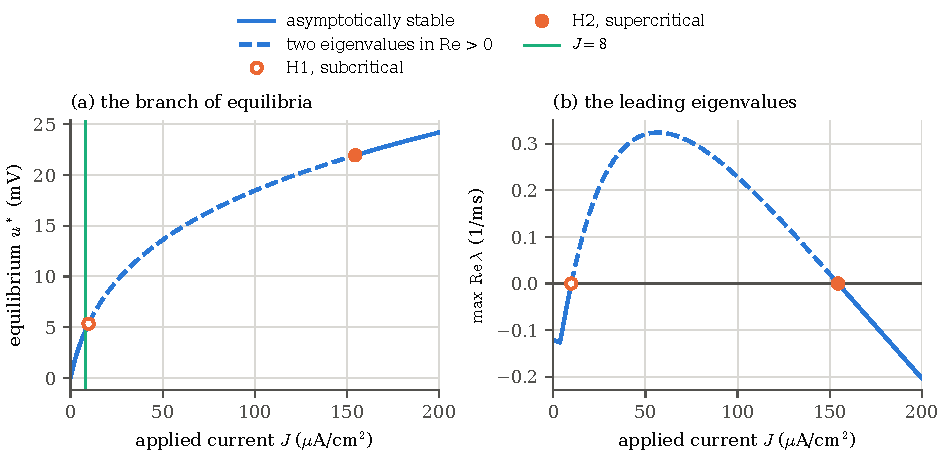
\includegraphics[width=\textwidth]{figures/branch.pdf}
\caption{The branch of equilibria at $E_l = 10.613$ (\texttt{code/hh\_make\_figures.py}). (a) $u^*(J)$ for $J \in [0, 200]$, solid where the equilibrium is asymptotically stable and dashed where it has two eigenvalues with positive real part; circles: the Hopf points of Theorem~\ref{thm:hopf}; the vertical line is $J = 8$, the current of Theorems~\ref{thm:ball} and~\ref{thm:three}. (b) The largest real part of an eigenvalue. The curves are floating-point evaluations; the positions of the Hopf points and the stability types are those proved in Theorem~\ref{thm:hopf}.}\label{fig:branch}
\end{figure}

\begin{corollary}[computer-assisted, with the cited Theorem~\ref{thm:kuz}]\label{cor:hopf}
Let $E_l \in [10.59, 10.62]$. Near $(x^*(J_{Hi}), J_{Hi})$ the one-parameter family \eqref{eq:hh}, with parameter $J$, is locally topologically equivalent to the suspension of the Hopf normal form by a two-dimensional stable node, with $\sigma = +1$ at $J_{H1}$ and $\sigma = -1$ at $J_{H2}$ (Theorem~\ref{thm:kuz}). Consequently, in the neighbourhood where the equivalence holds:
\begin{enumerate}
\item[(a)] (subcritical) for $J < J_{H1}$ close to $J_{H1}$, where the equilibrium is stable, there is a limit cycle, and it is not orbitally stable; for $J \ge J_{H1}$ close to $J_{H1}$ there is none;
\item[(b)] (supercritical) for $J < J_{H2}$ close to $J_{H2}$, where the equilibrium is unstable, there is an orbitally asymptotically stable limit cycle; for $J \ge J_{H2}$ close to $J_{H2}$ there is none.
\end{enumerate}
\end{corollary}

The corollary is local: it gives no bound on how far from $J_{Hi}$ the cycles persist. That the saddle-type orbit of Theorem~\ref{thm:three}(b) at $J = 8$ belongs to the family born at $J_{H1}$ is numerical evidence only (Section~\ref{sec:numerics}).

\begin{theorem}[computer-assisted]\label{thm:ball}
Let $J = 8$. For every $E_l \in [10.59, 10.62]$ the system \eqref{eq:hh} has a periodic orbit $\Gamma(E_l)$ that crosses $\Sigma_{20}$ with $\dot u > 0$ once per period, whose minimal period lies in $[\TballLo, \TballHi]$~ms, along which $u$ reaches at least $\UballMax$~mV, and whose nontrivial Floquet multipliers satisfy $|\mu| \le \Normball$. It is orbitally asymptotically stable. Its point on $\Sigma_{20}$ is the only fixed point of the first-return map in a box with half-widths at most about $\PieceBoxRad$ that contains it (Section~\ref{sec:proofs-orbits}).
\end{theorem}

So the firing frequency $1000/T$ lies in $[\FreqLo, \FreqHi]$~Hz. Figure~\ref{fig:period}(a) shows the period enclosures.

\begin{theorem}[computer-assisted]\label{thm:three}
Let $J = 8$ and let $E_l$ be one of $10.613$, $\ELs$ and $10.599$. At $\ELs$ the statement holds for every $E_l$ in the program's ball about $\ELs$, of radius below $10^{-25}$, which Arb prints as the decimal ball $\ELstarBiPrinted$ (a larger ball that contains it).
\begin{enumerate}
\item[(a)] There is a periodic orbit $\Gamma_s$ through $\Sigma_{20}$, crossed with $\dot u > 0$, with minimal period $T_s$ and nontrivial multipliers $\mu_1$, $\mu_2$, $\mu_3$ as in Table~\ref{tab:stable}; $\mu_1$ is enclosed in a disc that holds exactly one multiplier. $u$ reaches at least $\SmaxLoHH$, $\SmaxLoStar$ and $\SmaxLoGO$~mV along $\Gamma_s$ (in the order of the three values of $E_l$). $\Gamma_s$ is orbitally asymptotically stable.
\item[(b)] There is a periodic orbit $\Gamma_u$ through $\Sigma_5$, crossed with $\dot u > 0$, with minimal period $T_u$ and multipliers as in Table~\ref{tab:unstable}: $\mu_1$ is real and larger than $1$, $|\mu_2| < 1$ and $|\mu_3| < 1$. $\Gamma_u$ is of saddle type and not orbitally stable, and $u \le \UmaxHiHH$, $\UmaxHiStar$ and $\UmaxHiGO$~mV along it.
\item[(c)] $\Gamma_s$, $\Gamma_u$ and the equilibrium are three distinct invariant sets. The section point of $\Gamma_s$ is the only fixed point of the first-return map in a box with half-widths at most about $\SboxRadHH$ that contains it, and that of $\Gamma_u$ in a box with half-widths from about $\UboxRadMinHH$ to $\UboxRadHH$ (at $E_l = 10.613$; these are the Krawczyk boxes of the proof, and Section~\ref{sec:proofs-orbits} gives them at the other two values). Table~\ref{tab:points} gives enclosures of the section points, not boxes of uniqueness. Nothing is claimed about other periodic orbits.
\end{enumerate}
\end{theorem}

\begin{table}[t]
\centering\small
\caption{Theorem~\ref{thm:three}(a), the stable orbit $\Gamma_s$ on $\Sigma_{20}$ at $J = 8$: the minimal period (ms) and the nontrivial Floquet multipliers. Every bound is rounded outward from the program's balls (\texttt{data/certify\_bistability.txt}, stages 4 and 7).}\label{tab:stable}
\begin{tabular}{@{}llll@{}}
\toprule
$E_l$ & $T_s$ & $\mu_1$ & bound on $|\mu_2|$, $|\mu_3|$ \\
\midrule
\TabStableRows
\bottomrule
\end{tabular}

\bigskip
\caption{Theorem~\ref{thm:three}(b), the saddle-type orbit $\Gamma_u$ on $\Sigma_5$ at $J = 8$.}\label{tab:unstable}
\footnotesize\setlength{\tabcolsep}{4pt}
\begin{tabular}{@{}lllll@{}}
\toprule
$E_l$ & $T_u$ & $\mu_1$ (real) & $\mu_2$ & bound on $|\mu_3|$ \\
\midrule
\TabUnstableRows
\bottomrule
\end{tabular}

\bigskip
\caption{Enclosures of the section points $(m, n, h)$ of Theorem~\ref{thm:three}: each lies in the product of the three intervals, an outward rounding of the set $K$ of the proof (Section~\ref{sec:proofs-orbits}). Uniqueness is proved only in the Krawczyk boxes of Theorem~\ref{thm:three}(c), which are about $10^{2}$ to $10^{4}$ times narrower.}\label{tab:points}
\footnotesize
\begin{tabular}{@{}llll@{}}
\toprule
orbit, $E_l$ & $m$ & $n$ & $h$ \\
\midrule
$\Gamma_s$, $10.613$ & $\SptmHH$ & $\SptnHH$ & $\SpthHH$\\
$\Gamma_s$, $\ELs$ & $\SptmStar$ & $\SptnStar$ & $\SpthStar$\\
$\Gamma_s$, $10.599$ & $\SptmGO$ & $\SptnGO$ & $\SpthGO$\\
$\Gamma_u$, $10.613$ & $\UptmHH$ & $\UptnHH$ & $\UpthHH$\\
$\Gamma_u$, $\ELs$ & $\UptmStar$ & $\UptnStar$ & $\UpthStar$\\
$\Gamma_u$, $10.599$ & $\UptmGO$ & $\UptnGO$ & $\UpthGO$\\
\bottomrule
\end{tabular}
\end{table}

\begin{corollary}[computer-assisted]\label{cor:bist}
For $J = 8$ and every $E_l \in [10.59, 10.62]$, equivalently for $E_l = 10.613$ and every $J \in [\JequivLo, \JequivHi]$, the system \eqref{eq:hh} has a locally asymptotically stable equilibrium and an orbitally asymptotically stable periodic orbit. At $E_l = 10.613$, $\ELs$ and $10.599$ it also has a periodic orbit of saddle type.
\end{corollary}

\begin{corollary}[computer-assisted]\label{cor:ident}
Let $J = 8$ and let $E_l$ be $10.613$, $10.599$ or a value in the ball about $\ELs$ of Theorem~\ref{thm:three}. The stable orbit $\Gamma_s$ of Theorem~\ref{thm:three}(a) is the orbit $\Gamma(E_l)$ of Theorem~\ref{thm:ball}: its section point lies in the interior of the box of Theorem~\ref{thm:ball} for each of the pieces of the $E_l$ interval that contain $E_l$ (two pieces for $10.613$ and $10.599$, which are ends of pieces, and one for $\ELs$).
\end{corollary}

\begin{remark}[what is not claimed]\label{rem:not}
We do not claim that the equilibrium and $\Gamma(E_l)$ are the only attractors, nor anything about their basins, nor that $\Gamma_u$ lies on the boundary between the basins; numerically it does lie on a separatrix \cite[p.~62]{lxr2023}. The orbits are unique only in their boxes; at the three values of Theorem~\ref{thm:three} the stable orbits of Theorems~\ref{thm:ball} and~\ref{thm:three} are the same (Corollary~\ref{cor:ident}), and at other values of $E_l$ we have not compared them with anything. Nothing is proved about periodic orbits at currents other than $J = 8$ (and those equivalent to it by Lemma~\ref{lem:shift}), about the fold of cycles that numerically bounds the bistable range from below, or about the equilibria for $J \ge \JssBoundHigh$.
\end{remark}

\begin{figure}[t]
\centering
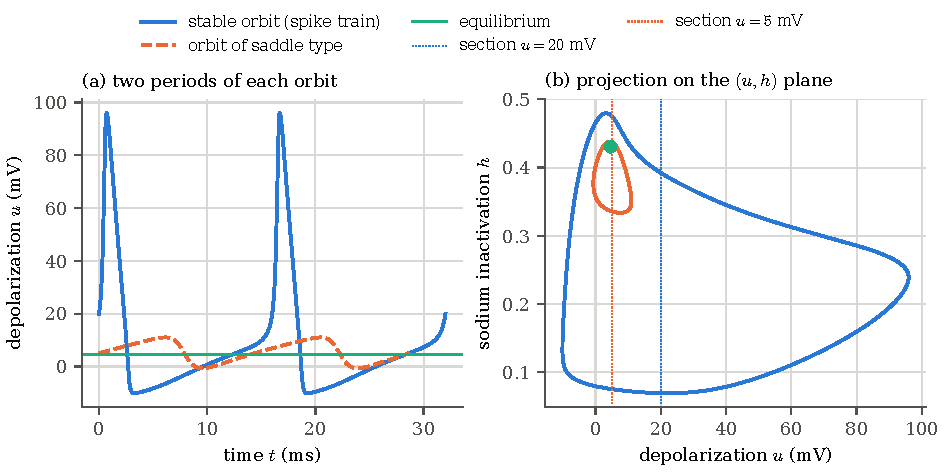
\includegraphics[width=\textwidth]{figures/orbits.pdf}
\caption{The orbits of Theorem~\ref{thm:three} at $J = 8$, $E_l = 10.613$, integrated in floating point from the high-precision section points of Section~\ref{sec:numerics} (\texttt{code/hh\_make\_figures.py}). (a) $u(t)$ over two periods of the stable orbit $\Gamma_s$ (solid) and of the saddle-type orbit $\Gamma_u$ (dashed), and the equilibrium $u^*$. (b) The projection on the $(u, h)$ plane, with the sections $u = 20$ and $u = 5$ (dotted) and the equilibrium (dot). The enclosures of the theorems are far narrower than the lines.}\label{fig:orbits}
\end{figure}

\section{Proofs for the branch of equilibria}\label{sec:proofs-eq}

\subsection{Lemmas}

\begin{lemma}[proved]\label{lem:quartic}
Let $p(\lambda) = \lambda^4 + a_1\lambda^3 + a_2\lambda^2 + a_3\lambda + a_4$ be real with $a_1, a_3, a_4 > 0$, $D_2 = a_1a_2 - a_3$ and $D_3 = a_3D_2 - a_1^2a_4$.
\begin{enumerate}
\item[(a)] $p$ has a root on the imaginary axis if and only if $D_3 = 0$. In that case, with $\omega = \sqrt{a_3/a_1} > 0$, $p(\lambda) = (\lambda^2 + \omega^2)(\lambda^2 + a_1\lambda + a_4/\omega^2)$, the roots $\pm i\omega$ are simple and the other two roots have negative real part.
\item[(b)] If $D_3 > 0$, then $D_2 > 0$ and every root has negative real part.
\item[(c)] If $D_3 < 0$, then exactly two roots, counted with multiplicity, have positive real part.
\end{enumerate}
\end{lemma}

\begin{proof}
(a) $p(0) = a_4 \ne 0$. For real $\omega \ne 0$, $p(i\omega) = \omega^4 - a_2\omega^2 + a_4 + i\omega(a_3 - a_1\omega^2)$, so $p(i\omega) = 0$ if and only if $\omega^2 = a_3/a_1$ and $\omega^4 - a_2\omega^2 + a_4 = 0$; with $\omega^2 = a_3/a_1$ the second condition reads $(a_3^2 - a_1a_2a_3 + a_1^2a_4)/a_1^2 = -D_3/a_1^2 = 0$. Expanding $(\lambda^2 + \omega^2)(\lambda^2 + a_1\lambda + c)$ gives $\lambda^4 + a_1\lambda^3 + (c + \omega^2)\lambda^2 + a_1\omega^2\lambda + c\omega^2$; with $c = a_4/\omega^2$ the last two coefficients are $a_3$ and $a_4$, and $c + \omega^2 = a_2$ is equivalent to $a_1^2a_4 + a_3^2 = a_1a_2a_3$, that is $D_3 = 0$. The quadratic $\lambda^2 + a_1\lambda + a_4/\omega^2$ has positive coefficients, so its roots have negative real part; it does not vanish at $\pm i\omega$, so these roots are simple.

(b), (c) If $D_3 > 0$ then $a_3D_2 = D_3 + a_1^2a_4 > 0$, so $D_2 > 0$. Let $Q = \{(a_1, \ldots, a_4) : a_1, a_3, a_4 > 0\}$ and $N(a)$ the number of roots of $p$ in $\{\re\lambda > 0\}$. The roots of a monic polynomial depend continuously on its coefficients, so $N$ is locally constant on the set of coefficient vectors for which no root lies on the imaginary axis (a root can enter or leave the open right half-plane only through the axis). By (a) this set, within $Q$, is $\{D_3 \ne 0\}$. Now $D_3 > 0$ is equivalent to $a_2 > \theta(a_1, a_3, a_4) := a_3/a_1 + a_1a_4/a_3$, a continuous function on $(0, \infty)^3$, so $Q \cap \{D_3 > 0\}$ is connected, and so is $Q \cap \{D_3 < 0\} = \{a_2 < \theta\}$. Hence $N$ is constant on each. $(\lambda + 1)^4$ has $(a_1, a_2, a_3, a_4) = (4, 6, 4, 1)$, $D_3 = 64 > 0$ and $N = 0$; $(\lambda^2 - \lambda + 1)(\lambda^2 + 3\lambda + 1) = \lambda^4 + 2\lambda^3 - \lambda^2 + 2\lambda + 1$ has $D_3 = -12 < 0$ and $N = 2$, the roots of $\lambda^2 - \lambda + 1$ having real part $1/2$ and those of $\lambda^2 + 3\lambda + 1$ being negative.
\end{proof}

\begin{lemma}[proved]\label{lem:linstab}
If every eigenvalue of $A = Df(x_0)$ at an equilibrium $x_0$ of a $C^2$ vector field has negative real part, $x_0$ is locally asymptotically stable.
\end{lemma}

\begin{proof}
There are $K, \gamma > 0$ with $\|e^{At}\| \le Ke^{-\gamma t}$, so $P = \int_0^\infty e^{A^Tt}e^{At}\,dt$ exists, is symmetric positive definite and satisfies $A^TP + PA = -I$ (integrate $\frac{d}{dt}e^{A^Tt}e^{At}$). Write $f(x_0 + y) = Ay + g(y)$ with $|g(y)| \le L|y|^2$ for $|y| \le 1$ and put $V(y) = y^TPy$. Along solutions $\dot V = -|y|^2 + 2y^TPg(y) \le -|y|^2/2$ for $|y| \le r_0 = \min(1, 1/(4L\|P\|))$. With $\lambda_{\min}|y|^2 \le V \le \lambda_{\max}|y|^2$ ($\lambda$ the extreme eigenvalues of $P$), the set $\{V < \lambda_{\min} r_0^2\}$ lies in $\{|y| < r_0\}$, is positively invariant, and on it $\dot V \le -V/(2\lambda_{\max})$, so $V(y(t)) \le V(y(0))e^{-t/(2\lambda_{\max})} \to 0$. This gives stability and attraction.
\end{proof}

\begin{lemma}[proved]\label{lem:unstab}
If $A = Df(x_0)$ at an equilibrium $x_0$ of a $C^2$ vector field has an eigenvalue with positive real part, $x_0$ is not stable.
\end{lemma}

\begin{proof}
Let $4\gamma > 0$ be the smallest positive real part of an eigenvalue of $A$, and split $\R^n = E_+ \oplus E_-$ into the invariant subspaces of the eigenvalues with positive and with nonpositive real part, $A = \operatorname{diag}(A_+, A_-)$ in adapted coordinates $y = (y_+, y_-)$. For a real matrix all of whose eigenvalues have real part at least $4\gamma$ (at most $0$) there is an inner product with $\langle A_+v, v\rangle \ge 3\gamma|v|^2$ (with $\langle A_-v, v\rangle \le \gamma|v|^2$): use a basis in which the matrix is in real Jordan form with off-diagonal entries scaled below $\gamma$. With these inner products on $E_\pm$, put $V(y) = |y_+|^2 - |y_-|^2$ and write $f(x_0 + y) = Ay + g(y)$, $|g(y)| \le L|y|^2$. Then $\dot V \ge 6\gamma|y_+|^2 - 2\gamma|y_-|^2 - 4L|y|^3$. On the cone $\{V > 0\}$, $|y| \le \sqrt2|y_+|$, so $\dot V \ge 4\gamma|y_+|^2 - 4\sqrt8L|y_+|^3 \ge 2\gamma|y_+|^2 \ge 2\gamma V$ when $|y| \le r_0$ for a suitable $r_0 > 0$. A solution starting in the cone with $|y(0)|$ arbitrarily small stays in it while $|y| \le r_0$, and $V$ grows at least like $e^{2\gamma t}$ there, so it leaves the ball of radius $r_0$.
\end{proof}

\begin{lemma}[proved]\label{lem:psi}
(a) $|B_n|/n! \le 4/(2\pi)^n$ for every $n \ge 0$. Hence, for a real ball $X$ with $|x| \le r < 3$ on $X$ and $0 \le k < N + 2 - (N + 2)r/(2\pi)$, the $k$-th Taylor coefficient of $\Psi$ at $x \in X$ is $\sum_{n=k}^{N} \frac{B_n}{n!}\binom{n}{k} x^{n-k} + \theta$ with $|\theta| \le \frac{4\binom{N+1}{k} r^{N+1-k}}{(2\pi)^{N+1}(1 - \rho)}$, $\rho = \frac{N+2}{N+2-k}\cdot\frac{r}{2\pi}$.
(b) $E(w) = (e^w - 1)/w = 1/\Psi(w)$ is entire and positive on $\R$, and its Taylor coefficients $e_j(w) = E^{(j)}(w)/j!$ satisfy $e_j(w) = \frac{1}{j!}\int_0^1 s^j e^{sw}\,ds = {}_1F_1(j + 1; j + 2; w)/(j + 1)!$. Each $e_j$ is strictly increasing in $w$, so on an interval $[w_-, w_+]$ it lies between $e_j(w_-)$ and $e_j(w_+)$.
\end{lemma}

\begin{proof}
(a) $\Psi(x) = \sum_n B_n x^n/n!$ for $|x| < 2\pi$ \cite[eq.~24.2.1]{dlmf} with $B_0 = 1$, $B_1 = -1/2$ and $B_n = 0$ for odd $n \ge 3$ \cite[Sect.~24.2]{dlmf}. For even $n \ge 2$, $|B_n|/n! = 2\zeta(n)/(2\pi)^n$ \cite[eq.~25.6.2]{dlmf} and $\zeta(n) \le \zeta(2) = \pi^2/6$, so $|B_n|/n! \le (\pi^2/3)/(2\pi)^n < 4/(2\pi)^n$; for $n = 0, 1$ the bound reads $1 \le 4$ and $1/2 \le 2/\pi$. Differentiating the series $k$ times, the tail $n > N$ of the $k$-th coefficient is bounded by $\sum_{n > N} 4\binom{n}{k} r^{n-k}/(2\pi)^n$, whose ratio of consecutive terms, $\frac{n+1}{n+1-k}\cdot\frac{r}{2\pi}$, does not increase with $n$ and is at most $\rho < 1$ for $n \ge N + 1$; a geometric series gives the bound.
(b) $E(w) = \int_0^1 e^{sw}\,ds$ is entire and positive for real $w$, so $e_j(w) = \frac{1}{j!}\int_0^1 s^je^{sw}\,ds$, and its derivative $\frac{1}{j!}\int_0^1 s^{j+1}e^{sw}\,ds$ is positive. Expanding $e^{sw}$, $\int_0^1 s^je^{sw}\,ds = \sum_{k \ge 0}\frac{w^k}{k!(j+k+1)}$, while ${}_1F_1(j+1; j+2; w) = \sum_{k\ge0}\frac{(j+1)_k}{(j+2)_k}\frac{w^k}{k!} = \sum_{k \ge 0}\frac{j+1}{j+1+k}\frac{w^k}{k!}$ by the definition of Kummer's function \cite[eq.~13.2.2]{dlmf}.
\end{proof}

The program for Theorems~\ref{thm:eq} and \ref{thm:hopf} (\file{code/hh_ball.py}) evaluates $\Psi$ through (a) with $N = 240$ where $|x| < 3$ and through its closed form elsewhere, where it refuses any ball containing $0$; the program for Theorems~\ref{thm:ball} and \ref{thm:three} (\file{code/hh_arb.py}) evaluates the Taylor coefficients of $E$ through (b), with ${}_1F_1$ from Arb \cite{johansson2019}, and those of $\Psi$ as the reciprocal series. The two implementations give overlapping enclosures of $\ELs$ (the self-test of \file{data/certify_equilibria_hopf.txt}, part 0).

\paragraph{The first Lyapunov coefficient.} Let $A$ have a simple pair of eigenvalues $\pm i\omega$, $\omega > 0$, let $Aq = i\omega q$, $A^Tp = -i\omega p$ and $\langle p, q\rangle = \bar p^Tq = 1$, and write the Taylor expansion of the vector field at the equilibrium $x_0$ as $f(x_0 + y) = Ay + \frac12B(y, y) + \frac16C(y, y, y) + O(|y|^4)$ with symmetric multilinear $B$ and $C$. Then
\begin{equation}\label{eq:l1}
  \ell_1 = \frac{1}{2\omega}\re\Bigl(\langle p, C(q, q, \bar q)\rangle - 2\langle p, B(q, A^{-1}B(q, \bar q))\rangle + \langle p, B(\bar q, (2i\omega I - A)^{-1}B(q, q))\rangle\Bigr),
\end{equation}
as given by Kuznetsov \cite[Sect.~``First Lyapunov Coefficient'']{kuznetsov2006}, who cites his book \cite{kuznetsov2004} for it; the bifurcation theorem itself goes back to Hopf \cite{hopf1943}, cited here as a credit only. We use it through the following theorem.

\begin{citedtheorem}[cited: {\cite[Sects.~``Two-dimensional Case'', ``Multi-dimensional Case'' and ``First Lyapunov Coefficient'']{kuznetsov2006}}]\label{thm:kuz}
Let $\dot x = f(x, \alpha)$, $x \in \R^n$, $\alpha \in \R$, with $f$ smooth, have a family of equilibria $x^0(\alpha)$ whose Jacobian $A(\alpha)$ has one pair of complex eigenvalues $\mu(\alpha) \pm i\omega(\alpha)$ with $\mu(0) = 0$, $\omega(0) = \omega_0 > 0$, and at $\alpha = 0$ a simple pair $\pm i\omega_0$, $n_s$ eigenvalues with negative and $n_u$ with positive real part, $n_s + n_u + 2 = n$. If $\ell_1(0) \ne 0$ (computed by \eqref{eq:l1} at $\alpha = 0$) and $\mu'(0) \ne 0$, the system is locally topologically equivalent near the origin to the suspension of the normal form
\[
 \dot y_1 = \beta y_1 - y_2 + \sigma y_1(y_1^2 + y_2^2), \quad \dot y_2 = y_1 + \beta y_2 + \sigma y_2(y_1^2 + y_2^2), \quad \dot y^s = -y^s, \quad \dot y^u = y^u,
\]
$y^s \in \R^{n_s}$, $y^u \in \R^{n_u}$, $\sigma = \operatorname{sign}\ell_1(0)$. For $\sigma = +1$ the origin of the planar normal form is asymptotically stable for $\beta < 0$ and unstable for $\beta \ge 0$, and a unique limit cycle, unstable, exists for $\beta < 0$; for $\sigma = -1$ the origin is asymptotically stable for $\beta \le 0$ and unstable for $\beta > 0$, and a unique limit cycle, stable, exists for $\beta > 0$.
\end{citedtheorem}

The implementation of \eqref{eq:l1} is tested on systems whose $\ell_1$ is known independently: the planar formula of Guckenheimer and Holmes as printed in \cite{kuznetsov2006}, and the following four-dimensional system, whose $\ell_1$ we compute through the centre manifold.

\begin{lemma}[proved]\label{lem:testsys}
For $\omega, a, e > 0$ and real $\varsigma, b, c, d, \phi$, the system
\[
\begin{aligned}
\dot x_1 &= -\omega x_2 + \varsigma x_1 r^2 + c\, x_1x_3 + \phi\, x_1x_4, & \dot x_3 &= -a x_3 + b r^2,\\
\dot x_2 &= \omega x_1 + \varsigma x_2 r^2 + c\, x_2x_3 - \phi\, x_2x_4, & \dot x_4 &= -e x_4 + d(x_1^2 - x_2^2),
\end{aligned}
\qquad r^2 = x_1^2 + x_2^2,
\]
has, at the origin and with $q = p = (1, -i, 0, 0)/\sqrt2$, the first Lyapunov coefficient $\ell_1 = \frac{2}{\omega}\bigl(\varsigma + \frac{bc}{a} + \frac{d\phi e}{2(e^2 + 4\omega^2)}\bigr)$, that is, $\ell_1 = \re c_1/\omega$ where $c_1$ is the coefficient of $w|w|^2$ in the equation on the centre manifold in the coordinate $w$ with $x = wq + \bar w\bar q + O(|w|^2)$.
\end{lemma}

\begin{proof}
With $z = x_1 + ix_2$, the linear part is $\dot z = i\omega z$ on the centre subspace. A centre manifold is a graph $x_3 = h_3(z)$, $x_4 = h_4(z)$ with $h_{3,4} = O(|z|^2)$; its quadratic parts solve the homological equations. For $h_3 = \eta_3|z|^2$: $\frac{d}{dt}|z|^2 = 0$ along the linear flow, so $-a\eta_3|z|^2 + b|z|^2 = 0$, $\eta_3 = b/a$. For $h_4 = \re(\kappa z^2)$: $\frac{d}{dt}\re(\kappa z^2) = \re(2i\omega\kappa z^2)$ along the linear flow and $x_1^2 - x_2^2 = \re(z^2)$, so $2i\omega\kappa = -e\kappa + d$, $\kappa = d/(e + 2i\omega)$. On the manifold, $\dot z = \dot x_1 + i\dot x_2 = i\omega z + \varsigma z|z|^2 + c\,z h_3 + \phi\,\bar z h_4 + O(|z|^4)$, because $x_1x_4 - ix_2x_4 = \bar z x_4$, and the terms of $h_{3,4}$ of order three contribute only at order four. Since $\phi\bar z\,\re(\kappa z^2) = \frac{\phi}{2}(\kappa z^2\bar z + \bar\kappa\bar z^3)$, the coefficient of $z^2\bar z$ is $\varsigma + cb/a + \phi\kappa/2$. There are no quadratic terms, so this is the resonant cubic coefficient in $z$. With $x = wq + \bar w\bar q$ on the centre subspace we have $z = \sqrt2\,w$, so the coefficient in $w$ is $c_1 = 2(\varsigma + cb/a + \phi\kappa/2)$, and $\re c_1/\omega = \frac{2}{\omega}(\varsigma + \frac{bc}{a} + \frac{\phi}{2}\re\kappa)$ with $\re\kappa = de/(e^2 + 4\omega^2)$. Evaluating \eqref{eq:l1} directly gives the same value: $\langle p, C(q, q, \bar q)\rangle = 4\varsigma$, $B(q, \bar q) = (0, 0, 2b, 0)$, $\langle p, B(q, A^{-1}B(q, \bar q))\rangle = -2bc/a$, $B(q, q) = (0, 0, 0, 2d)$ and $\langle p, B(\bar q, (2i\omega - A)^{-1}B(q, q))\rangle = 2d\phi/(e + 2i\omega)$.
\end{proof}

The program runs the implementation of \eqref{eq:l1} on two planar test systems and on the system of Lemma~\ref{lem:testsys} with $(\omega, \varsigma, a, b, c, d, e, \phi) = (1, -\tfrac1{10}, 2, \tfrac13, \tfrac12, \tfrac32, \tfrac12, 1)$ and with $\omega = \tfrac32$, $\varsigma = -\tfrac15$; the known values of $\ell_1$ are $\TestPlanarA$, $\TestPlanarB$, $\TestCoupledA$ and $\TestCoupledB$, of both signs, and the implementation reproduces each to within $10^{-60}$. Two mutated versions, with $+2$ in place of $-2$ in the middle term and with $(-A)^{-1}$ in place of $(2i\omega I - A)^{-1}$, give $\MutSign$ and $\MutTwoiw$ on the first coupled system and are refused (negative controls).

\subsection{Proofs}

All references to checks are to \file{data/certify_equilibria_hopf.txt}, written by \file{code/certify_equilibria_hopf.py} at $256$ bits; the model is \file{code/hh_ball.py}, which evaluates every quantity as a truncated power series in $u$ over complex balls, so that a series evaluated on a ball $U$ encloses the Taylor coefficients of the quantity at every point of $U$. The leak potential enters as the ball $[10.605 \pm 0.015] \supset [10.59, 10.62]$.

\begin{proof}[Proof of Proposition~\ref{prop:elstar}]
$I(x^*(0)) = 0$ is linear in $E_l$ and gives the formula. The program evaluates it in ball arithmetic and prints the resulting ball, of radius below $10^{-38}$ (part 0 of the output, the line that begins ``E\_l* ='', which also gives the current at $u = 0$); that ball is the step of the proof, and $\ELstar$ is its outward rounding. The ball computed by the independent implementation of \file{code/hh_arb.py} overlaps it; that comparison is a self-test, not a step of the proof. The current at $u = 0$ for $E_l = 10.613$ is $I(x^*(0)) = g_l(\ELs - 10.613)$, since $I$ depends on $E_l$ only through $-g_lE_l$.
\end{proof}

\begin{proof}[Proof of Theorem~\ref{thm:eq}]
By Lemma~\ref{lem:basic}(d) we must count the solutions of $\Jss(u) = J$. For $u < -12$ each of the three terms of $\Jss(u) = g_{\mathrm{Na}}m^3h(u - 115) + g_Kn^4(u + 12) + g_l(u - E_l)$ is negative (Lemma~\ref{lem:basic}(a) and $E_l > -12$), so $\Jss(u) < 0 \le J$. For $u \ge 115$ the first term is nonnegative, the third positive, and the second at least $g_{\mathrm{K}} n_\infty(115)^4 \cdot 127$ by Lemma~\ref{lem:basic}(b); the program encloses this number and finds it at least $\JssBoundHigh > 200$ (part A, third check). On $[-12, 115]$ the program shows $\Jss' > 0$ on each of $\NpiecesSlope$ pieces of a subdivision (part A, first check), so $\Jss$ is strictly increasing there, and it shows $\Jss(-12) \le \JssMinusTwelve < 0$ and $\Jss(115) > 200$ (fourth check) for every $E_l$ in the ball. For $J \in [0, 200]$ the intermediate value theorem and monotonicity give exactly one solution, and it lies in $(-12, 115)$. $\Jss$ is real-analytic with positive derivative there, so its inverse $u^*$ is real-analytic and increasing.
\end{proof}

\begin{proof}[Proof of Theorem~\ref{thm:hopf}]
\emph{Signs along the branch.} The program subdivides $[-12, 115]$ into $\NpiecesHurwitz$ pieces and shows on each that $a_1$, $a_3$, $a_4 > 0$ and that $D_3 > 0$ or $D_3 < 0$, except on $\Nundecided$ pieces of width below $10^{-5}$ (part B, first check). These undecided pieces form two clusters, $\ClusterOne$ and $\ClusterTwo$ (second check); every zero of $D_3$ in $[-12, 115]$ lies in them. On each cluster, slightly enlarged, the program encloses $dD_3/du$ in $\dDthreeOne$ and $\dDthreeTwo$ respectively and shows that $D_3$ has opposite signs at the two ends (third and fifth checks), so each cluster contains exactly one zero, and it is simple. Interval Newton steps $N(X) = m - D_3(m)/D_3'(X)$, $m$ the midpoint of $X$, are applied as long as $N(X) \subset X$; by the mean value theorem the zero $u_H \in X$ satisfies $u_H = m - D_3(m)/D_3'(\xi)$ for some $\xi \in X$, so it stays in the new box, which gives $u_{H1}$ and $u_{H2}$ in balls of radius at most $\uHOnerad$ and $\uHTworad$ (fourth and sixth checks; Theorem~\ref{thm:hopf} prints them rounded outward to $12$ decimals). The program shows $D_3 > 0$ at $u = -12$ and $u = 115$ and $D_3 < 0$ at a point between the zeros (seventh check), which fixes the signs on the three intervals.

\emph{(a) and (b).} By Theorem~\ref{thm:eq} the equilibrium at current $J$ has $u^*(J) \in (-12, 115)$, and $u^*(J) < u_{H1}$ exactly when $J < J_{H1}$, since $u^*$ is increasing; similarly for $u_{H2}$. Lemma~\ref{lem:quartic}(b) gives the stable ranges, and Lemma~\ref{lem:linstab} local asymptotic stability; Lemma~\ref{lem:quartic}(c) and (a) give the count on $(J_{H1}, J_{H2})$ and the absence of roots on the axis, and Lemma~\ref{lem:unstab} the instability; Lemma~\ref{lem:quartic}(a) gives (b), with $\omega_i^2 = a_3/a_1$ at $u_{Hi}$, enclosed by the program. The program also checks, as a guard against coding errors, that $a_2 - \omega^2 - a_4/\omega^2$ encloses $0$ at $u_{Hi}$ and that the Routh array at the midpoint of $(u_{H1}, u_{H2})$ has two sign changes; both are consequences of Lemma~\ref{lem:quartic}, not steps of the proof.

\emph{(c).} $J_{Hi} = \Jss(u_{Hi})$ is evaluated on the ball of $u_{Hi}$ for each value of $E_l$, and for $\ELs$ on its ball; Lemma~\ref{lem:shift} gives the affine dependence and the range over $[10.59, 10.62]$, whose ends are the values at $10.62$ and $10.59$ (part C).

\emph{(d).} The coefficients $a_k$ are real-analytic in $u$, and $i\omega_i$ is a simple root of $p(\cdot\,; u_{Hi})$, so by the implicit function theorem there is an analytic root $\lambda(u)$ with $\lambda(u_{Hi}) = i\omega_i$ and $\lambda'(u) = -\partial_up/\partial_\lambda p$. The program encloses $\re\lambda'(u_{Hi})$ in $\dluOne$ and $\dluTwo$, and $\Jss'(u_{Hi})$ in $\dJuOne$ and $\dJuTwo$; the eigenvalue as a function of $J$ is $\lambda(u^*(J))$, with derivative $\lambda'(u)/\Jss'(u)$, enclosed as stated.

\emph{(e).} By Lemma~\ref{lem:jac}(c) with $\lambda = i\omega_i$, the closed-form vectors $q$ and $w$ satisfy $Aq = i\omega q$ and $w^TA = i\omega w^T$ (the program also checks that the residuals enclose $0$). The program normalizes $\langle q, q\rangle = 1$ and $w^Tq = 1$, and puts $p = \bar w$, so that $A^Tp = -i\omega p$ and $\langle p, q\rangle = 1$. It obtains $B$ and $C$ from the vector field evaluated as a power series in $t$ along $x^*(u_{Hi}) + tv$: the coefficients of $t^2$ and $t^3$ are $\frac12B(v, v)$ and $\frac16C(v, v, v)$, and $B(v, v')$, $C(q, q, \bar q)$ follow by polarization. $A^{-1}$ and $(2i\omega I - A)^{-1}$ are applied by Arb's rigorous linear solver. $\ell_1$ does not depend on $J$ or $E_l$, which enter $f$ additively. The resulting enclosures exclude $0$ (part C). A non-rigorous recomputation with SymPy derivatives and mpmath eigenvectors agrees to a relative $\CrossrelOne$ and $\CrossrelTwo$.
\end{proof}

\begin{proof}[Proof of Corollary~\ref{cor:hopf}]
Fix $E_l$ and $i$, and put $\alpha = J - J_{Hi}$, $x^0(\alpha) = x^*(u^*(J))$, which is an analytic family of equilibria by Theorem~\ref{thm:eq}. By Theorem~\ref{thm:hopf}(b) the Jacobian at $\alpha = 0$ has a simple pair $\pm i\omega_i$, $n_s = 2$ and $n_u = 0$; the pair continues analytically as $\mu(\alpha) \pm i\omega(\alpha)$ with $\mu'(0) = \re\lambda'(J_{Hi}) \ne 0$ by (d), and $\ell_1(0) \ne 0$ by (e). Theorem~\ref{thm:kuz} applies with $\sigma = +1$ at $H1$ and $\sigma = -1$ at $H2$. The topological equivalence of the families maps equilibria to equilibria, preserves their asymptotic stability, maps periodic orbits to periodic orbits, and preserves orbital asymptotic stability and its failure, since these are defined through neighbourhoods and limits along orbits. At $H1$ the equilibrium is asymptotically stable exactly for $J < J_{H1}$ near $J_{H1}$ (Theorem~\ref{thm:hopf}(a)), and in the normal form with $\sigma = +1$ exactly for $\beta < 0$; so these parameter sets correspond, and the unstable cycle of the normal form for $\beta < 0$ gives (a); the suspension by $\dot y^s = -y^s$ keeps it not orbitally stable. At $H2$ the equilibrium is unstable exactly for $J < J_{H2}$ near $J_{H2}$ and, with $\sigma = -1$, the origin exactly for $\beta > 0$; the stable cycle there, attracting also in the $y^s$ directions, gives (b).
\end{proof}

\section{Validated integration and Poincar\'e maps}\label{sec:integration}

This section states and proves what the program \file{code/certify_bistability.py} relies on; the implementation is \file{code/hh_lohner.py} (integrator and Poincar\'e maps), \file{code/certlib.py} (Krawczyk, Gershgorin, the equilibrium) and \file{code/ball_stable.py} (the contraction on the $E_l$ interval), with the model in \file{code/hh_arb.py}. The program extends \eqref{eq:hh} by $E_l$ as a fifth variable with $\dot E_l = 0$, so that an interval of $E_l$ is a direction of the initial set. We write $F$ for this analytic vector field on $\R^5$, $\varphi_t$ for its flow, and, for $y \in \R^5$,
\[
  x_k(y) = \frac{1}{k!}\frac{d^k}{dt^k}\varphi_t(y)\Big|_{t=0}, \qquad A_k(y) = \frac{1}{k!}\frac{d^k}{dt^k}D\varphi_t(y)\Big|_{t=0} = Dx_k(y).
\]
The $x_k$ follow from the recursion $x_{k+1} = [F(x(\cdot))]_k/(k+1)$, $[\cdot]_k$ the $k$-th Taylor coefficient in $t$, and the $A_k$ from $A_0 = I$, $A_{k+1} = \frac{1}{k+1}\sum_{i \le k}[DF(x(\cdot))]_iA_{k-i}$ (the variational equation $\dot V = DF(x(t))V$). The program evaluates both recursions in ball arithmetic on a box $X$, with the Taylor coefficients of the rate functions from exact formulas for the exponentials, from Lemma~\ref{lem:psi}(b) for $\Psi$, and from the reciprocal series of $1 + e^{(30-u_0)/10}e^{-(u - u_0)/10}$ for $\beta_h$, where $u_0$ is the voltage about which the series is expanded. By the inclusion property of ball arithmetic this gives boxes $x_k(X) \ni x_k(y)$ and $A_k(X) \ni A_k(y)$ for all $y \in X$. For intervals we write $[0, h]^k = [0, h^k]$.

\subsection{One step}

\begin{lemma}[proved; the a priori enclosure]\label{lem:apriori}
Let $X$ and $Y$ be boxes, $h > 0$, $p \ge 1$, and suppose $\sum_{k \le p} x_k(X)[0, h]^k + x_{p+1}(Y)[0, h]^{p+1} \subset \inter Y$. Then for every $y \in X$ the solution $\varphi_s(y)$ exists and lies in $Y$ for $s \in [0, h]$, and $\varphi_s(y) \in \sum_{k \le p}x_k(y)s^k + x_{p+1}(Y)s^{p+1}$.
\end{lemma}

\begin{proof}
The left side contains $X$ (the term $k = 0$ is $X$ and the others contain $0$), so $X \subset \inter Y$. Let $y \in X$ and $s_1 = \sup\{s \in [0, h] : \varphi_\sigma(y) \in Y$ for $\sigma \in [0, s]\}$. For $s \le s_1$ Taylor's theorem with the Lagrange remainder, applied to each component of the analytic function $t \mapsto \varphi_t(y)$, gives $\varphi_s(y)_i = \sum_{k \le p}x_k(y)_is^k + x_{p+1}(\varphi_\xi(y))_is^{p+1}$ for some $\xi \in (0, s)$, because $\frac{1}{(p+1)!}\frac{d^{p+1}}{dt^{p+1}}\varphi_t(y)|_{t = \xi} = x_{p+1}(\varphi_\xi(y))$ by the group property. Since $\varphi_\xi(y) \in Y$, $\varphi_s(y)$ lies in the left side of the hypothesis, hence in $\inter Y$. If $s_1 < h$, the solution would stay in $Y$ a little beyond $s_1$ (it is in the open set $\inter Y$ at $s_1$), a contradiction; so $s_1 = h$ and the solution, which stays in a compact set, exists on $[0, h]$.
\end{proof}

\begin{lemma}[proved; the variational enclosure]\label{lem:var}
With $X$, $Y$, $h$, $p$ as in Lemma~\ref{lem:apriori}, let $W$ be a box of $5 \times 5$ matrices with $\sum_{k \le p}A_k(X)[0, h]^k + A_{p+1}(Y)\,W\,[0, h]^{p+1} \subset \inter W$ entrywise. Then $D\varphi_s(y) \in W$ and $D\varphi_s(y) \in N(s) := \sum_{k \le p}A_k(X)s^k + A_{p+1}(Y)\,W\,s^{p+1}$ for $y \in X$, $s \in [0, h]$.
\end{lemma}

\begin{proof}
Differentiating $D\varphi_{s + \sigma}(y) = D\varphi_\sigma(\varphi_s(y))D\varphi_s(y)$ $k$ times in $\sigma$ at $\sigma = 0$ gives
\[
 \frac{1}{k!}\frac{d^k}{ds^k}D\varphi_s(y) = A_k(\varphi_s(y))\,D\varphi_s(y).
\] The argument of Lemma~\ref{lem:apriori}, entrywise, with $\varphi_\xi(y) \in Y$ from that lemma and $D\varphi_\xi(y) \in W$ up to $s_1$, proves the claim; $D\varphi_0 = I$ lies in the left side, hence in $\inter W$.
\end{proof}

\begin{lemma}[proved; the mean-value form]\label{lem:mv}
With $X$ convex, $\bar y \in X$ and the hypotheses of Lemma~\ref{lem:apriori}, for every $y \in X$ and $s \in [0, h]$ there is a matrix $\tilde M$ in $M(s) := \sum_{k \le p}A_k(X)s^k$ such that $\varphi_s(y) - \sum_{k \le p}x_k(\bar y)s^k - \tilde M(y - \bar y) \in x_{p+1}(Y)s^{p+1}$.
\end{lemma}

\begin{proof}
$T(y) = \sum_{k \le p}x_k(y)s^k$ has $DT(y) = \sum_{k \le p}A_k(y)s^k$. By the mean value theorem on the segment from $\bar y$ to $y$, $T_i(y) - T_i(\bar y) = DT_i(\zeta_i)(y - \bar y)$ with $\zeta_i \in X$, and the row $DT_i(\zeta_i)$ lies in row $i$ of $M(s)$. Lemma~\ref{lem:apriori} bounds $\varphi_s(y) - T(y)$.
\end{proof}

\paragraph{Sets.} The program represents a set of initial points as $S = \{\bar x + C\rho_0 + B\rho : \rho_0 \in r_0, \rho \in r\}$ with an exact point $\bar x$, exact matrices $C$, $B$ and boxes $r_0$, $r$ (the doubleton sets of Zgliczy\'nski \cite{zgliczynski2002}, after Lohner \cite{lohner1987}), and a set of matrices as $\{\bar V + B_VR : R \in R_V\}$. One step to time $s$, with $X \supset S$ and $\tilde M$ as in Lemma~\ref{lem:mv}, computes: $a = \sum_{k \le p}x_k(\bar x)s^k + x_{p+1}(Y)s^{p+1}$, $\bar M = $ the midpoint of $M(s)$, $C' = $ the midpoint of $\bar MC$, $Z = a + (M(s) - \bar M)(Cr_0 + Br) + (\bar MC - C')r_0$, $\bar x' = $ the midpoint of $Z$, a matrix $B'$ from a floating-point QR decomposition, a ball enclosure of $B'^{-1}$, and $r' = (B'^{-1}\bar MB)r + B'^{-1}(Z - \bar x')$; the box $r_0$ is kept. The program keeps $0 \in r_0$ and $0 \in r$: an initial set has $r = 0$ and $r_0$ a box centred at $0$ (the half-widths of the initial box on the section, and the $E_l$ ball minus its midpoint), and the update gives $0 \in r'$ because $0 \in r$ and $0 \in Z - \bar x'$, $\bar x'$ being the midpoint of $Z$. Hence $\bar x \in S \subset X$, and Lemma~\ref{lem:mv} applies with $\bar y = \bar x$.

\begin{lemma}[proved]\label{lem:lohner}
If $y = \bar x + C\rho_0 + B\rho \in S$, then $\varphi_s(y) = \bar x' + C'\rho_0 + B'\rho'$ for some $\rho' \in r'$. The same holds for the matrix sets: if $D\varphi_t(x_0) = \bar V + B_VR$, $R \in R_V$, and $D\varphi_s(\varphi_t(x_0)) \in N(s)$, the program's update gives $D\varphi_{t+s}(x_0) = \bar V' + B_V'R'$ with $R' \in R_V'$.
\end{lemma}

\begin{proof}
By Lemma~\ref{lem:mv}, $\varphi_s(y) = \alpha + \tilde M(C\rho_0 + B\rho)$ with $\alpha \in a$ and $\tilde M \in M(s)$. Then $\varphi_s(y) = \zeta + C'\rho_0 + \bar MB\rho$ with $\zeta = \alpha + (\tilde M - \bar M)(C\rho_0 + B\rho) + (\bar MC - C')\rho_0 \in Z$, and $\varphi_s(y) = \bar x' + C'\rho_0 + B'\rho'$ with $\rho' = B'^{-1}\bar MB\rho + B'^{-1}(\zeta - \bar x') \in r'$, all inclusions being those of ball arithmetic. For matrices, $\tilde N(\bar V + B_VR) = \bar N\bar V + (\tilde N - \bar N)(\bar V + B_VR) + \bar NB_VR$ with $\tilde N \in N(s)$ and $\bar N$ its midpoint, and the same rearrangement applies.
\end{proof}

\subsection{Crossing a section}

Let $\Sigma = \{x_i = c\}$ and $g(x) = x_i - c$ (the sections here are crossed with $\dot x_i > 0$). The Poincar\'e routine (\file{code/hh_lohner.py}, \texttt{poincare}) starts from a set $S_0$ whose hull lies exactly on $\Sigma$ (otherwise it stops: \texttt{check\_on\_section}), and integrates step by step, classifying every step by the a priori box $Y$ of the step, an enclosure $F_i(Y)$ of $\dot x_i$ on $Y$, and the hull $X$ of the set at the start of the step:
\begin{enumerate}
\item[(D)] \emph{departure}: while the hull meets $\Sigma$, every step must have $F_i > 0$ on $Y$;
\item[(N)] \emph{no crossing}: $g \ne 0$ on $Y$; or $F_i > 0$ on $Y$ and $g > 0$ on $X$; or $F_i > 0$ on $Y$ and $g < 0$ on the hulls at both ends of the step;
\item[(P)] \emph{pass}: $F_i < 0$ on $Y$ (counted as a downward pass);
\item[(H)] \emph{hit}: $F_i > 0$ on $Y$, $g < 0$ on $X$, and times $0 \le s_- < s_+ \le h$ with $g < 0$ on the enclosure of the set at time $s_-$ and $g > 0$ at time $s_+$.
\end{enumerate}

\begin{lemma}[proved; first hit and the crossing]\label{lem:hit}
Suppose a run from $S_0 \subset \Sigma$ consists of steps of types (D), (N), (P) followed by one step of type (H) that ends at the total time $t_0 + s_+$. For $y \in S_0$ let $\tau(y)$ be the smallest $t > 0$ with $g(\varphi_t(y)) = 0$ and $\frac{d}{dt}g(\varphi_t(y)) > 0$. Then $\tau(y)$ exists and lies in $t_0 + (s_-, s_+)$, every $t \in (0, \tau(y))$ with $g(\varphi_t(y)) = 0$ has $\frac{d}{dt}g(\varphi_t(y)) < 0$, and there are at most as many such $t$ as steps of type (P). Moreover, with $Y_T \supset \varphi_{[t_0 + s_-, t_0 + s_+]}(S_0)$ and any $s_m \in [s_-, s_+]$, the point $P(y) = \varphi_{\tau(y)}(y)$ satisfies, for each $j$,
\[
 P_j(y) = \varphi_{t_0 + s_m}(y)_j - q_j\,\bigl(\varphi_{t_0 + s_m}(y)_i - c\bigr), \qquad \tau(y) = t_0 + s_m - \frac{\varphi_{t_0 + s_m}(y)_i - c}{\bar F_i},
\]
with $q_j$ in the interval of values of $F_j/F_i$ on $Y_T$ and $\bar F_i$ in the interval of values of $F_i$ on $Y_T$.
\end{lemma}

\begin{proof}
On a step with $F_i > 0$ on $Y$ the function $t \mapsto g(\varphi_t(y))$ is strictly increasing, and on a step with $F_i < 0$ strictly decreasing, since $\frac{d}{dt}g(\varphi_t(y)) = F_i(\varphi_t(y))$ and $\varphi_t(y) \in Y$ (Lemma~\ref{lem:apriori}). In the departure phase $g(\varphi_0(y)) = 0$ and $g$ increases, so $g > 0$ for $t > 0$ until the hull leaves $\Sigma$. A step of type (N) has no zero of $g$: either $g \ne 0$ on $Y$, or $g$ increases from a positive value, or $g$ increases and is negative at both ends. A step of type (P) has at most one zero, with negative derivative. On the step of type (H), $g$ is negative at the start and increasing, negative at $s_-$ and positive at $s_+$, so it has exactly one zero, in $(s_-, s_+)$, with positive derivative. This proves the first part. For the formulas, $\varphi_{\tau}(y)_j - \varphi_{t_0 + s_m}(y)_j = \int F_j\,dt$ and $c - \varphi_{t_0 + s_m}(y)_i = \int F_i\,dt$ over the arc between the two times, which lies in $Y_T$; since $F_i > 0$ on $Y_T$, the first integral is $\int (F_j/F_i)F_i\,dt$, a weighted mean of $F_j/F_i$ times the second, and the second is the length of the time interval times a mean of $F_i$.
\end{proof}

The program evaluates these formulas on the Lohner representation of $\varphi_{t_0 + s_m}(S_0)$ (Lemma~\ref{lem:lohner}), so that the time shift and the displacement along the flow cancel to first order, intersects the result with $Y_T$, and records the extremes of $u$ over the step enclosures; the ``$u$ reaches at least'' bounds of the theorems are maxima over step times of lower bounds of $u$ on the set, so every orbit from $S_0$ attains them.

\begin{lemma}[proved; the derivative]\label{lem:dp}
Under the hypotheses of Lemma~\ref{lem:hit}, every $y \in S_0$ has a neighbourhood $W$ in $\Sigma$ and a real-analytic $\tilde\tau$ on $W$ with $\tilde\tau = \tau$ on $S_0 \cap W$; so $\tau$ and $P$ are analytic on $S_0$ in this sense, and $DP(y) = \bigl(I - F(P(y))e_i^T/F_i(P(y))\bigr)D\varphi_{\tau(y)}(y)$ on the tangent space of $\Sigma$. If $D\varphi_{t_0}(y) \in \bar V + B_VR_V$ and $N(T)$ is the enclosure of Lemma~\ref{lem:var} over $T = [s_-, s_+]$, then $DP(y)$ lies in $(I - F(\mathcal P)e_i^T/F_i(\mathcal P))\,N(T)\,(\bar V + B_VR_V)$, where $\mathcal P$ is the enclosure of $P(S_0)$.
\end{lemma}

\begin{proof}
$G(t, z) = g(\varphi_t(z))$ has $\partial_tG(\tau(y), y) = F_i(P(y)) > 0$, so the implicit function theorem gives an analytic $\tilde\tau$ near $y$ with $\tilde\tau(y) = \tau(y)$ and $G(\tilde\tau(z), z) = 0$. For $z \in S_0$ near $y$, $\tilde\tau(z)$ lies in the window $t_0 + (s_-, s_+)$ of the step of type (H), where $t \mapsto G(t, z)$ is strictly increasing (proof of Lemma~\ref{lem:hit}); its only zero there is $\tau(z)$, so $\tilde\tau(z) = \tau(z)$. Differentiating, $D\tilde\tau = -e_i^TD\varphi_{\tilde\tau}/F_i(P)$ and $DP = D\varphi_{\tilde\tau} + F(P)D\tilde\tau$. The enclosure follows from $D\varphi_{\tau}(y) = D\varphi_{\tau - t_0}(\varphi_{t_0}(y))D\varphi_{t_0}(y)$ and Lemmas~\ref{lem:var} and~\ref{lem:lohner}.
\end{proof}

Since $E_l$ is constant along the flow, Lemmas~\ref{lem:hit} to~\ref{lem:period} hold as well for the flow of \eqref{eq:hh} at each fixed $E_l$ of the $E_l$ range of $S_0$, with $S_0$ replaced by its slice at that $E_l$; this is how they are applied below. In the coordinates $(m, n, h)$ of $\Sigma_{20}$ or $\Sigma_5$ and for fixed $E_l$, the matrix of $DP$ is the block of rows and columns $m$, $n$, $h$ of the $5 \times 5$ matrix of the lemma; its row $u$ vanishes.

\begin{lemma}[proved; minimal period]\label{lem:period}
Under the hypotheses of Lemma~\ref{lem:hit}, if $y \in S_0$ and $P(y) = y$, the orbit of $y$ is periodic with minimal period $\tau(y)$. If moreover $S_0$ contains a neighbourhood of $y$ in $\Sigma$, then on a neighbourhood of $y$ the map $P$ is the local return map at $y$ of Section~\ref{sec:model}.
\end{lemma}

\begin{proof}
$\varphi_{\tau(y)}(y) = y$, and $y$ is not an equilibrium because $F_i(y) > 0$ (departure condition). The periods of a nonconstant periodic orbit are the integer multiples of its minimal period $T_0$. If $T_0 < \tau(y)$, then $\varphi_{T_0}(y) = y \in \Sigma$ with $\frac{d}{dt}g = F_i(y) > 0$ at $t = T_0 \in (0, \tau(y))$, which Lemma~\ref{lem:hit} excludes. For the second statement, the function $\tilde\tau$ of Lemma~\ref{lem:dp} at $y$ and the return time $\tau_{\mathrm{loc}}$ of the local return map are both the solution given by the implicit function theorem at $(t, z) = (\tau(y), y)$, which is unique near that point, so they agree near $y$, and $\tilde\tau = \tau$ on $S_0$.
\end{proof}

\begin{lemma}[proved; Floquet multipliers]\label{lem:floquet}
Let $\Gamma$ be a periodic orbit with minimal period $T$ of an analytic vector field $F$ on $\R^d$, through $y \in \Sigma$ with $F_i(y) \ne 0$, let $M = D\varphi_T(y)$, and let $P$ be the local return map at $y$ (Section~\ref{sec:model}). Then $DP(y) = \Pi M$ on the tangent space $E = \{v : v_i = 0\}$ of $\Sigma$, with $\Pi = I - F(y)e_i^T/F_i(y)$, and $\det(\lambda I - M) = (\lambda - 1)\det(\lambda I - DP(y))$.
\end{lemma}

\begin{proof}
$MF(y) = F(y)$, and $F(y) \notin E$. Differentiating $x_i(\varphi_{\tau_{\mathrm{loc}}(z)}(z)) = c$ at $z = y$, where $\tau_{\mathrm{loc}}(y) = T$ and $\varphi_T(y) = y$, gives $D\tau_{\mathrm{loc}}(y) = -e_i^TM/F_i(y)$ on $E$, so $DP(y) = M + F(y)D\tau_{\mathrm{loc}}(y) = \Pi M$ on $E$, where $\Pi$ is the projection onto $E$ along $F(y)$. For $v \in E$, $Mv = \Pi Mv + \frac{e_i^TMv}{F_i(y)}F(y)$, so in a basis consisting of $F(y)$ and a basis of $E$ the matrix of $M$ is block upper triangular with diagonal blocks $1$ and $DP(y)$.
\end{proof}

\subsection{Fixed points, multipliers and stability}

\begin{citedtheorem}[cited: {\cite[Theorem~13.3]{rump2010}}, a form of the test of Krawczyk \cite{krawczyk1969} and Moore \cite{moore1977}]\label{thm:krawczyk}
Let $f : D \to \R^n$ be continuously differentiable, $\tilde x \in \R^n$, $X$ a box, and $R$ a real $n \times n$ matrix, with $0 \in X$ and $\tilde x + X \subset D$. Suppose
\[
  S(X, \tilde x) := -Rf(\tilde x) + \bigl(I - R\,Jf(\tilde x + X)\bigr)X \subset \inter X,
\]
where $Jf(Y)$ is the interval hull of the Jacobians of $f$ at the points of $Y$. Then $R$ and all matrices $M \in Jf(\tilde x + X)$ are nonsingular, and there is a unique root $\hat x$ of $f$ in $\tilde x + S(X, \tilde x)$.
\end{citedtheorem}

This is the theorem as Rump states it, with his notation $Jf(Y) = \hull\{Jf(y) : y \in Y\}$ \cite[eq.~(13.3)]{rump2010}; the proof there ends by noting that the nonsingularity makes $f$ injective on $\tilde x + X$. We use it through the following lemma.

\begin{lemma}[proved]\label{lem:kraw}
Let $G$ be continuously differentiable on a box $\bar z + X$ with $0 \in X$, $R$ a real matrix, $\mathcal G$ a box containing $G(\bar z)$ and $\mathbf M$ an interval matrix containing $DG(z)$ for every $z \in \bar z + X$. If $K := \bar z - R\mathcal G + (I - R\mathbf M)X \subset \inter(\bar z + X)$, then $G$ has exactly one zero in $\bar z + X$, and it lies in $K$.
\end{lemma}

\begin{proof}
$Jf(\bar z + X)$, for $f = G$, is the smallest box of matrices containing every $DG(z)$, so it lies in $\mathbf M$, and by the inclusion property of interval arithmetic $\bar z + S(X, \bar z) \subset K \subset \inter(\bar z + X)$, that is $S(X, \bar z) \subset \inter X$. Theorem~\ref{thm:krawczyk} with $D = \bar z + X$ gives a zero $\hat x \in \bar z + S(X, \bar z) \subset K$ and the nonsingularity of every matrix in $Jf(\bar z + X)$. If $G(z_1) = G(z_2)$ with $z_1, z_2 \in \bar z + X$, then $0 = \tilde M(z_1 - z_2)$ with $\tilde M = \int_0^1 DG(z_2 + t(z_1 - z_2))\,dt$; each entry of $\tilde M$ is a mean of the same entry of Jacobians at points of the convex box $\bar z + X$, so $\tilde M \in Jf(\bar z + X)$ is nonsingular and $z_1 = z_2$.
\end{proof}

The program (\file{code/certlib.py}, \texttt{krawczyk}) applies the lemma to $G = P - \mathrm{id}$ on a box $Z = \bar z + X$ of $\Sigma$, with $R$ the floating-point inverse of the midpoint of $\mathbf{DP}(Z) - I$: it computes $K = \bar z - R(\mathcal P(\bar z) - \bar z) + (I - R(\mathbf{DP}(Z) - I))X$ with an enclosure $\mathcal P(\bar z)$ of $P(\bar z)$ and an enclosure $\mathbf{DP}(Z)$ of $DP$ over $Z$, and checks $K \subset \inter Z$.

\begin{lemma}[proved; Gershgorin discs]\label{lem:gersh}
Let $\mathbf M$ be a real interval matrix, $S$ an invertible complex matrix, and $D_i = \{z : |z - c_i| \le R_i\}$ discs with $R_i \ge |(S^{-1}MS)_{ii} - c_i| + \sum_{j \ne i}|(S^{-1}MS)_{ij}|$ for every $M \in \mathbf M$. Then for every $M \in \mathbf M$: (a) every eigenvalue lies in $\bigcup_iD_i$; (b) a union of $k$ discs that is disjoint from the other discs contains exactly $k$ eigenvalues, counted with multiplicity; (c) if $D_1$ is disjoint from the others and $c_1$ is real, the eigenvalue in $D_1$ is real.
\end{lemma}

\begin{proof}
(a) Gershgorin's theorem \cite{gershgorin1931} for $S^{-1}MS$, whose discs lie in the $D_i$: if $S^{-1}MSv = \lambda v$ and $|v_i|$ is maximal, $|\lambda - (S^{-1}MS)_{ii}| \le \sum_{j \ne i}|(S^{-1}MS)_{ij}|$. (b) Let $\Delta$ be the diagonal of $S^{-1}MS$ and $M_t = \Delta + t(S^{-1}MS - \Delta)$, $t \in [0, 1]$. The Gershgorin discs of $M_t$ have the same centres and $t$ times the radii, so they lie in the $D_i$, and by (a) no eigenvalue of $M_t$ crosses the boundary of the union of the $k$ discs. The eigenvalues depend continuously on $t$; at $t = 0$ they are the centres of these discs, the diagonal entries of $S^{-1}MS$, and exactly $k$ of them lie in the union. (c) $M$ is real, so $\bar\lambda$ is an eigenvalue with $\bar\lambda \in D_1$ when $\lambda \in D_1$; by (b) $D_1$ contains only one eigenvalue, so $\lambda = \bar\lambda$.
\end{proof}

The program takes $S$ from the floating-point eigenvectors of the midpoint of $\mathbf M$, encloses $S^{-1}$ and $S^{-1}\mathbf MS$ in ball arithmetic, and for a real eigenvalue of the midpoint takes a real eigenvector, so that $c_1$ is real (\file{code/certlib.py}, \texttt{gershgorin\_eigenbasis} and \texttt{multiplier\_test}).

\begin{lemma}[proved; contraction]\label{lem:contr}
Let $Z \subset \R^3$ be a box, $P : Z \to \inter Z$ of class $C^1$ with $\|DP(z)\|_\infty \le \kappa < 1$ for $z \in Z$. Then $P$ has exactly one fixed point $z^*$ in $Z$, $P^k(z) \to z^*$ for $z \in Z$, and every eigenvalue of $DP(z^*)$ has modulus at most $\kappa$.
\end{lemma}

\begin{proof}
$Z$ is convex, so $\|P(z) - P(z')\|_\infty \le \kappa\|z - z'\|_\infty$ by the mean value inequality, and Banach's fixed point theorem applies on the complete set $Z$. The spectral radius is at most any induced norm.
\end{proof}

\begin{lemma}[proved; orbital asymptotic stability]\label{lem:oas}
Let $\Gamma$ be a periodic orbit with minimal period $T$ of an analytic vector field $F$ on $\R^d$, through $y^* \in \Sigma$ with $F_i(y^*) > 0$, let $P$ be the local return map at $y^*$, and suppose every eigenvalue of $DP(y^*)$ has modulus less than $1$. Then $\Gamma$ is orbitally asymptotically stable.
\end{lemma}

\begin{proof}
\emph{Step 1.} There is a norm $|\cdot|_*$ on the tangent space of $\Sigma$ with $|DP(y^*)|_* < 1$ (for a matrix of spectral radius $\rho$ and any $\eps > 0$ there is an induced norm with value less than $\rho + \eps$). By continuity of $DP$ and the mean value inequality there are $\kappa < 1$ and $\delta_0 > 0$ such that $B_0 = \{z \in \Sigma : |z - y^*|_* \le \delta_0\}$ is mapped into itself and $|P(z) - y^*|_* \le \kappa|z - y^*|_*$ there. Shrinking $\delta_0$, the return time $\tau_{\mathrm{loc}}$, which is continuous with $\tau_{\mathrm{loc}}(y^*) = T$, has values in $[T/2, 2T]$ on $B_0$.

\emph{Step 2.} (In the application $d = 4$, at fixed $E_l$.) By the implicit function theorem applied to $g(\varphi_t(x)) = 0$ at $(t, x) = (0, y^*)$, there are a neighbourhood $U$ of $y^*$ and a continuous $t_U$ on $U$ with $t_U(y^*) = 0$, $|t_U| \le T/4$ and $\pi(x) = \varphi_{t_U(x)}(x) \in \Sigma$; $\pi$ is continuous and $\pi(y^*) = y^*$. Given $\eta > 0$ and $\eps > 0$, let $U_\eta \subset U$ be a neighbourhood of $y^*$ with $\pi(U_\eta) \subset B_\eta = \{z \in \Sigma : |z - y^*|_* \le \eta\}$. The map $(t, x) \mapsto \varphi_t(x)$ is uniformly continuous on $[0, 3T] \times \{x : \dist(x, \Gamma) \le \delta_1\}$ for a small $\delta_1 > 0$, so there is $\delta \in (0, \delta_1]$ such that $|x - \gamma| < \delta$, $\gamma \in \Gamma$, implies $|\varphi_t(x) - \varphi_t(\gamma)| < \eps$ for $t \in [0, 3T]$ and $\varphi_{2T - s}(x) \in U_\eta$, where $\gamma = \varphi_s(y^*)$, $s \in [0, T)$ (because $\varphi_{2T - s}(\gamma) = y^*$). Such an $x$ stays within $\eps$ of $\Gamma$ up to the time $2T - s + t_U(\varphi_{2T-s}(x)) \in [3T/4, 9T/4]$, at which it lies in $B_\eta$.

\emph{Step 3.} Continuous dependence on initial data on $[0, 2T]$ gives $L$ with $|\varphi_t(z) - \varphi_t(y^*)| \le L|z - y^*|_*$ for $z \in B_0$, $t \in [0, 2T]$. For $z \in B_\eta$, $\eta \le \delta_0$, the iterates $P^k(z)$ stay in $B_\eta$ and tend to $y^*$, the return times $\tau_{\mathrm{loc}}(P^k(z))$ lie in $[T/2, 2T]$, and between the $k$-th and the next return the orbit stays within $L|P^k(z) - y^*|_* \le L\kappa^k\eta$ of $\Gamma$. Given $\eps$, choose $\eta \le \delta_0$ with $L\eta < \eps$ and then $\delta$ as in Step 2: every $x$ with $\dist(x, \Gamma) < \delta$ stays within $\eps$ of $\Gamma$ for all $t \ge 0$, and its distance to $\Gamma$ tends to $0$.
\end{proof}

\begin{lemma}[proved; saddle type]\label{lem:saddle}
Under the hypotheses of Lemma~\ref{lem:oas}, except that $DP(y^*)$ has a simple real eigenvalue $\mu_1 > 1$ and its other eigenvalues have modulus less than $1$, $\Gamma$ is not orbitally stable.
\end{lemma}

\begin{proof}
Choose coordinates $w = (\xi, \zeta) \in \R \times \R^2$ on $\Sigma$ centred at $y^*$ in which $DP(y^*) = \operatorname{diag}(\mu_1, B)$, and a norm $|\cdot|$ on $\R^2$ with $|B| \le \beta < 1$. Fix $\eps > 0$ with $\beta + \eps \le \mu_1 - \eps$ and $\mu_1 - \eps > 1$, and $\delta_0 > 0$ such that $P(w) = DP(y^*)w + r(w)$ with $\|r(w)\| \le \eps\|w\|$ for $\|w\| = \max(|\xi|, |\zeta|) \le \delta_0$. On the cone $\mathcal K = \{|\zeta| \le |\xi|\}$, $w' = P(w)$ satisfies $|\xi'| \ge (\mu_1 - \eps)|\xi|$ and $|\zeta'| \le \beta|\zeta| + \eps|\xi| \le |\xi'|$, so $w' \in \mathcal K$ and $\|w'\| \ge (\mu_1 - \eps)\|w\|$. Hence every $w \in \mathcal K \setminus \{0\}$, however close to $0$, has an iterate with $\|P^k(w)\| > \delta_0$ whose predecessor has norm at most $\delta_0$; by continuity of $P$, $\|P^k(w)\| \le \Lambda\delta_0$ for a constant $\Lambda$. Transversality gives $c_0 > 0$ and $\eta_0 > 0$ with $\dist(z, \Gamma) \ge c_0\|z\|$ for $z \in \Sigma$ with $\|z\| \le \eta_0$: for $|s| \le s_0$ small, the point $\varphi_s(y^*)$ of $\Gamma$ satisfies $|z - \varphi_s(y^*)| \ge |x_i(\varphi_s(y^*)) - c| \ge a|s|$ with $a = \frac12F_i(y^*)$, and $|z - \varphi_s(y^*)| \ge |z - y^*| - b|s|$ with $b = \max|F|$ near $\Gamma$, so $|z - \varphi_s(y^*)| \ge \frac{a}{a + b}|z - y^*|$; the rest of $\Gamma$ is at a positive distance from $y^*$, hence from $z$ when $z$ is close to $y^*$; and the norms are equivalent. Choosing $\delta_0$ with $\Lambda\delta_0 \le \eta_0$, orbits that start arbitrarily close to $\Gamma$ reach the distance $c_0\delta_0$ from it, and $\Gamma$ is not orbitally stable.
\end{proof}

\section{Proofs of Theorems~\ref{thm:ball} and \ref{thm:three} and Corollary~\ref{cor:bist}}\label{sec:proofs-orbits}

The references are to \file{data/certify_bistability.txt}; the program works at $\BiPrec$ bits with Taylor order $p = \BiOrder$ and a remainder tolerance $\BiTol$ relative to the scales $(100, 1, 1, 1, 10)$ of $(u, m, n, h, E_l)$. Every decimal bound it prints in stages 3 to 7 is rounded outward from its ball, and all $\BiLedger$ of them are read back as exact rationals and compared with the balls (stage 7, first check). Theorems~\ref{thm:ball} and \ref{thm:three} are the program's Theorems C and B; its Theorem A appears in the proof of Corollary~\ref{cor:bist}.

\begin{proof}[Proof of Theorem~\ref{thm:three}]
Fix $E_l$ as in the theorem. The program carries $E_l$ as a ball $\mathcal E$ that contains it: for $10.613$ and $10.599$ the ball of the decimal string at $96$ bits, of radius below $10^{-28}$, and for $\ELs$ a ball of radius below $10^{-25}$ (stage 3); every statement holds for each $E_l$ in $\mathcal E$. (a) The program computes a candidate $\bar z$ on $\Sigma_{20}$ by floating-point Newton steps, integrates the set $\{\bar z\} \times \mathcal E$ to its first return (a $C^0$ run) and the set $Z \times \mathcal E$, with the box $Z = \bar z + X$ of half-widths at most about $\SboxRadHH$ ($C^1$ run over $Z$; the half-widths are those at $E_l = 10.613$), each by a chain of steps as in Lemma~\ref{lem:hit}, and checks that the two runs integrated sets that contain $\{\bar z\} \times \mathcal E$ and $Z \times \mathcal E$ (``the C\textasciicircum{}0 run integrated a set containing \ldots''). It obtains enclosures of $P(\bar z)$ and of $DP$ over $Z$ (Lemma~\ref{lem:dp}), the latter with entries of radius about $\SDPradHH$, and verifies $K \subset \inter Z$ (stage 4, ``Krawczyk: unique fixed point of the first-return map in Z''). By Lemma~\ref{lem:kraw}, for every $E_l \in \mathcal E$ the map $P$ has exactly one fixed point $z^*$ in $Z$, and $z^* \in K$. By Lemma~\ref{lem:period} its orbit $\Gamma_s$ is periodic with minimal period $\tau(z^*)$, which lies in the enclosure of $\tau$ over $Z$ (Table~\ref{tab:stable}), and since $K \subset \inter Z$, near $z^*$ the map $P$ is the local return map at $z^*$. The Gershgorin discs of $\mathbf{DP}(Z)$ (Lemma~\ref{lem:gersh}) all lie in the open unit disc (``all nontrivial Floquet multipliers of the stable orbit lie in $|\mu| < 1$''), and the first is disjoint from the other two (``multiplier discs \ldots\ are isolated''), so it contains exactly one multiplier $\mu_1$ and the other two lie in the union of the others; Lemma~\ref{lem:floquet} identifies these eigenvalues with the nontrivial multipliers, and Lemma~\ref{lem:oas} gives orbital asymptotic stability. The run passes $\Sigma_{20}$ downward once and certifies the first return in $\SstepsHH$ steps; its step enclosures show that every orbit from $Z$ reaches $u \ge \SmaxLoHH$ (and the corresponding values at the other $E_l$).

(b) The same on $\Sigma_5$, with a box of half-widths from about $\UboxRadMinHH$ to $\UboxRadHH$: Lemma~\ref{lem:kraw} gives the fixed point, in $K \subset \inter Z$, and Lemma~\ref{lem:period} the period and the local return map; the three discs are pairwise disjoint, the first is centred on the positive real axis and lies outside the closed unit disc, and the other two lie inside the open unit disc (``exactly one Floquet multiplier of the second orbit is real and $> 1$''). By Lemma~\ref{lem:gersh}(b), (c), $\mu_1$ is real and larger than $1$, and $\Gamma_u$ is of saddle type; Lemma~\ref{lem:saddle} shows that it is not orbitally stable. The step enclosures bound $u \le \UmaxHiHH$ along every orbit from the box.

(c) $\Gamma_s$ reaches $u \ge \SmaxLoHH$ and $\Gamma_u$ stays below $\UmaxHiHH$ (at $E_l = 10.613$; similarly at the other values), so they are different (``the orbits are distinct''); neither is an equilibrium, because $\dot u > 0$ at their section points. Uniqueness holds in the Krawczyk boxes $Z$, whose largest half-widths are about $\SboxRadHH$, $\SboxRadStar$ and $\SboxRadGO$ for $\Gamma_s$ and $\UboxRadHH$, $\UboxRadStar$ and $\UboxRadGO$ for $\Gamma_u$ at the three values, and whose smallest half-widths for $\Gamma_u$ are about $\UboxRadMinHH$, $\UboxRadMinStar$ and $\UboxRadMinGO$ (stage 4, ``C\textasciicircum{}1 run over Z (radius \ldots)'', which prints the three half-widths; \file{data/identify_stable_orbit.txt} prints the centres of the boxes of $\Gamma_s$ exactly, and their half-widths, which are the printed floating-point radii rounded up to Arb's radius format, exactly as well). The fixed points lie in the sets $K$ (Lemma~\ref{lem:kraw}), and Table~\ref{tab:points} lists outward roundings of $K$, which are wider than $Z$.
\end{proof}

\begin{proof}[Proof of Theorem~\ref{thm:ball}]
Stage 4b cuts $[10.59, 10.62]$ into $\NPieces$ intervals of width $\PieceWidth$ and checks that they cover it without gaps (``the pieces cover [10.59, 10.62]''). For each piece $\mathcal E$ it chooses a box $Z$ on $\Sigma_{20}$, with half-widths at most about $\PieceBoxRad$, around an approximate fixed point, and runs two first-return computations over $Z \times \mathcal E$ as in Lemma~\ref{lem:hit}: a $C^0$ run that shows $P_{E}(Z) \subset \inter Z$ for every $E \in \mathcal E$, and a $C^1$ run that bounds $\|DP_{E}(z)\|_\infty$ for all $(z, E) \in Z \times \mathcal E$, by the maximum over the rows of the sums of the moduli of the entries of the enclosure; it also checks that both runs integrated sets that contain $Z \times \mathcal E$. Every piece passes with a bound between $\NormMin$ and $\NormMax$ (``every piece: $P_E(Z)$ in int $Z$, both runs integrated a set containing $Z \times$ piece, and sup $\|DP_E\|_\infty < 1$''; each line of a piece prints the three results). By Lemma~\ref{lem:contr}, $P_E$ has exactly one fixed point in $Z$, and every eigenvalue of $DP_E$ there has modulus at most $\Normball$; the fixed point lies in $P_E(Z) \subset \inter Z$, so by Lemma~\ref{lem:period} its orbit is periodic with minimal period in the enclosure of $\tau$ over $Z \times \mathcal E$ and near it $P_E$ is the local return map, and by Lemma~\ref{lem:oas} the orbit is orbitally asymptotically stable. $\Gamma(E_l)$ denotes this orbit. When $E_l$ is the common end of two pieces, each of the two boxes holds exactly one fixed point of $P_{E_l}$; we take $\Gamma(E_l)$ from the piece on the left (at $10.613$ and $10.599$ the two fixed points are the same point, by Corollary~\ref{cor:ident}). Each piece is carried as the ball $[\mathit{lo}, \mathit{hi}]$ of Arb, which contains the decimal interval. For the four pieces of Corollary~\ref{cor:ident} the boxes are recomputed, with the same printed lines, and printed exactly by \file{code/identify_stable_orbit.py}; for $E_l$ in those pieces $\Gamma(E_l)$ is taken from the printed boxes. The union over the pieces of the period enclosures is $[\TballLo, \TballHi]$, and the minimum over the pieces of the lower bounds of the maximum of $u$ is $\UballMax$ (stage 4b, last line, and stage 7).
\end{proof}

\begin{proof}[Proof of Corollary~\ref{cor:bist}]
By Theorem~\ref{thm:hopf}(c), $J_{H1} \ge \JHoneMinBall > 8$ for every $E_l \in [10.59, 10.62]$ (\file{data/certify_equilibria_hopf.txt}, part D), so by Theorems~\ref{thm:eq} and \ref{thm:hopf}(a) the equilibrium at $J = 8$ is unique and locally asymptotically stable. Theorem~\ref{thm:ball} gives the orbitally asymptotically stable periodic orbit, Theorem~\ref{thm:three}(b) the orbit of saddle type at the three values, and Lemma~\ref{lem:shift} the equivalent statement in $J$. The program for Theorems~\ref{thm:ball} and \ref{thm:three} proves the equilibrium part again, independently, at $96$ bits with the other implementation of $\Psi$ (its Theorem A, stage 3): an interval Newton step on $\Jss(u) - 8$ over $U = \EqNewtonU$ with $\Jss'(U) \subset \EqNewtonDF$ maps $U$ into its interior; $\Jss' > 0$ on $W = \EqW$ ($\EqWpieces$ pieces); $\Jss - 8$ has no zero on $[-12, 115] \setminus W$ ($\EqExcl$ interval evaluations) and none outside $[-12, 115]$ (the signs of Lemma~\ref{lem:basic}); the equilibrium lies in the box $u \in \EqBoxu$, $m \in \EqBoxm$, $n \in \EqBoxn$, $h \in \EqBoxh$; the enclosed characteristic polynomial has $a_1 \in \EqAOne$, $a_2 \in \EqATwo$, $a_3 \in \EqAThree$, $a_4 \in \EqAFour$, $D_2 \in \EqDtwo$ and $D_3 \in \EqDthree$; and four pairwise disjoint Gershgorin discs, centred at $\EqDiscOne$, $\EqDiscTwo \pm \EqDiscImTwo i$ and $\EqDiscFour$ with radii $\EqDiscROne$, $\EqDiscRTwo$ and $\EqDiscRFour$, lie in $\re\lambda < 0$.
\end{proof}

\begin{proof}[Proof of Corollary~\ref{cor:ident}]
The program \file{code/identify_stable_orbit.py} (output \file{data/identify_stable_orbit.txt}; $\IdChecks$ checks: $\IdProof$ proof checks, $\IdControls$ negative controls and $\IdCross$ cross-checks; about $\IdTime$~s with two worker processes) recomputes the fixed points of Theorem~\ref{thm:three}(a) as stage 4 of \file{code/certify_bistability.py} does, from the same floating-point candidate, and obtains the same sets $K$ (cross-checks). With the function and the arguments of stage 4b (the box centres predicted from the stage-4 run at $E_l = 10.613$ and its derivative $dz^*/dE_l$) it recomputes the boxes of Theorem~\ref{thm:ball} on the pieces \IdPieces, re-proves on each that $P_E(Z) \subset \inter Z$ and $\sup\|DP_E\|_\infty < 1$ for every $E_l$ in the piece, with runs that integrated sets containing $Z \times$ piece, and prints the centres of the boxes and their half-widths (the floating-point radii rounded up to Arb's radius format) exactly; its lines for these pieces are those of stage 4b in \file{data/certify_bistability.txt} (cross-checks). For each value and each of these pieces that contains it, it checks that the ball of the value lies in the piece and that $K$ lies in the interior of the box of the piece (the centre of $K$ is at most $\IdOffMax$ box radii from the centre of the box). The fixed point of Theorem~\ref{thm:three}(a) lies in $K$ (Lemma~\ref{lem:kraw}), hence in the box, where $P_E$ has exactly one fixed point (Lemma~\ref{lem:contr}); so it is the point of $\Gamma(E_l)$. As negative controls, $K$ at each value is tested against the box of a piece that does not contain the value, at least $\IdCtlMin$ box radii away, and against the box of its own piece with its half-widths shrunk to $0.1$ of their values; both inclusions fail, so the test is not loose by a factor of ten.
\end{proof}

\begin{figure}[t]
\centering
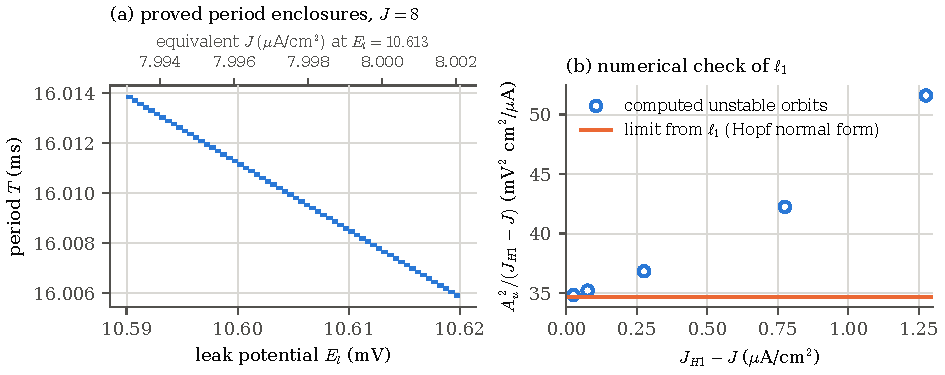
\includegraphics[width=\textwidth]{figures/period.pdf}
\caption{(a) Theorem~\ref{thm:ball}: the proved enclosures of the period of $\Gamma(E_l)$ on each of the $\NPieces$ pieces of the $E_l$ interval; the top axis gives the equivalent current at $E_l = 10.613$ (Lemma~\ref{lem:shift}). (b) Numerical: $A_u^2/(J_{H1} - J)$, where $A_u$ is the peak-to-peak amplitude of $u$ in mV, for the unstable periodic orbits computed in floating point at $J = 8.5$ to $9.75$ ($E_l = 10.613$; Table~\ref{tab:branch}), and its limit $16|q_u|^2\re\lambda'(J_{H1})/(\omega_1\ell_1) \in \SlopeOne$ predicted by the Hopf normal form from the proved values of Theorem~\ref{thm:hopf} (Section~\ref{sec:numerics}).}\label{fig:period}
\end{figure}

\section{The computer-assisted method}\label{sec:method}

\paragraph{Ball arithmetic.} All rigorous computations use Arb \cite{johansson2017} through python-flint $\FlintVersion$ (FLINT $\FLINTVersion$), in which a real number is a ball $[m \pm r]$ and a complex number a pair of balls. Every operation returns a ball that contains all results for all inputs in the input balls, and a comparison is true only if it holds for all points of the balls; an undecided comparison is false. The constants of \eqref{eq:hh} are exact rationals, converted to balls. Floating point (numpy, scipy, mpmath) proposes candidates, subdivision points, step sizes, the frames $B$ of the Lohner sets, the Krawczyk preconditioner and the eigenvector matrices of the Gershgorin discs; a bad choice can make a check fail but not succeed wrongly. The three programs print every check and stop at the first failed check, or at an exception, with a nonzero exit status and, once they have started, a line in their report that says so.

\paragraph{Printed bounds.} A bound printed as an interval $[a, b]$, or after $\le$ or $\ge$, is rounded outward from its ball in exact rational arithmetic (\file{code/outward.py}), and each program re-reads all of its printed bounds as rationals and compares them with the balls ($\HopfLedger$, $\BiLedger$ and $\IdLedger$ bounds). A ball printed as $[m \pm r]$ is Arb's own decimal enclosure. \file{code/hh_make_numbers.py} copies these bounds into the manuscript, or rounds them outward further, in exact rational arithmetic; no number of a theorem is typed by hand.

\paragraph{Checks.} Each program counts its checks by kind (Table~\ref{tab:checks}). A \emph{proof} check is a step of a proof above. A \emph{consistency} check verifies that an identity which a lemma proves exactly (such as $Aq = i\omega q$) holds within the enclosures. A \emph{negative control} feeds a deliberately wrong input to the code of a certificate, which must refuse it: for example, the Hopf factorization test at $u_{H1} + 10^{-3}$, where $a_2 - \omega^2 - a_4/\omega^2 \in \SplitControl$; mutated versions of \eqref{eq:l1}; Krawczyk on boxes shifted by ten box radii or by $10^{-9}$, and on the stable orbit's box with the vector field at $J = 8.05$ (the centre of $K$ lies $\CtlKJ$ box radii away); Krawczyk with the enclosure of $DP(Z)$ widened by $0.5$ in every entry, where the Newton point $\bar z - R(\mathcal P(\bar z) - \bar z)$ still lies in $Z$, so that the test must see the term $(I - R(\mathbf{DP}(Z) - I))X$; the check that the sets integrated contain $Z \times \mathcal E$, on a set a thousand times smaller than $Z$ and on a set with $E_l$ at the midpoint of its ball; an initial set on $u = 20$ with the crossing detected on $u = 19.999$; the equilibrium test at $J = 20$, where $D_3 \in \CtlTwentyDthree$; the contraction test on a box too small to contain the fixed points; on the usual box of a piece with the bound $1$ replaced by $0.5$, which the enclosure's upper bound $\CtlKappaHi$ of $\sup\|DP_E\|_\infty$ does not meet (so that the verdict is shown to use the bound); and on the saddle orbit, where every member of the enclosure has $\|DP\|_\infty \ge \CtlNorm$; the inclusion of $K$ of Theorem~\ref{thm:three}(a) in the box of Theorem~\ref{thm:ball} of a piece that does not contain the value of $E_l$, and in its own box shrunk to $0.1$; the integrator with the Taylor remainder set to $0$, and the a priori test on boxes that do not contain the motion; and wrong vector fields, among them $g_{\mathrm{Na}} = 120.0001$ against a high-precision reference solution. A \emph{self-test} compares the code with a known answer (exact solutions of test equations, the Poincar\'e map of a planar system with known multipliers, mpmath references for the Hodgkin--Huxley flow in three regimes, the test systems for $\ell_1$). \emph{Cross-checks} (a non-rigorous recomputation, such as $\ell_1$ from SymPy derivatives and mpmath eigenvectors, and $\re\lambda'(u_{Hi})$ and $\Jss'(u_{Hi})$ from central differences of mpmath eigenvalues, which agree with the enclosures to a relative $\TransrelOne$ and $\TransrelTwo$; or the comparison of a recomputed line with the committed output of another program) and \emph{numerical-only} checks enter no proof.

\begin{table}[t]
\centering\small
\caption{The checks of the three programs by kind, from their outputs.}\label{tab:checks}
\begin{tabular}{@{}lrrrrrrr@{}}
\toprule
program & all & proof & consistency & controls & self-tests & cross-checks & numerical \\
\midrule
\texttt{certify\_equilibria\_hopf.py} & $\HopfChecks$ & $\HopfProof$ & $\HopfConsistency$ & $\HopfControls$ & $\HopfSelftests$ & $\HopfCross$ & -- \\
\texttt{certify\_bistability.py} & $\BiChecks$ & $\BiProof$ & -- & $\BiControls$ & $\BiSelftests$ & -- & $\BiNumerical$ \\
\texttt{identify\_stable\_orbit.py} & $\IdChecks$ & $\IdProof$ & -- & $\IdControls$ & -- & $\IdCross$ & -- \\
\bottomrule
\end{tabular}
\end{table}

\paragraph{What an end-to-end run cannot show.} A certificate can pass although a rigorous ingredient is missing, when the true solution satisfies the inequalities with a wide margin. The controls were extended until the study below catches every mutation that is not marked weak. The program \file{code/mutation_study.py} makes deliberate mutations on copies of the programs, after running each unmutated program as a baseline (\file{data/mutation_study.txt}): of its $\MutTotal$ mutations, all $\MutStrong$ that are not marked weak stopped the program, $\MutByCheck$ of them at a failed check and $\MutByExc$ by an exception; the mutation marked weak, which changes a term of the order of the floating-point error of a root, far below the enclosure radii, passed ($\MutWeakPassed$ of $\MutWeak$). The study is not part of any proof, and a caught mutation shows only that the checks see that particular error. The tests of \eqref{eq:l1} in \file{code/certify_equilibria_hopf.py} were added for this paper.

\paragraph{Trust base.} The proofs assume that Arb and python-flint compute correct enclosures for the operations used (field operations, absolute values, complex conjugation, comparisons, \texttt{exp}, \texttt{sqrt}, the constant $\pi$, \texttt{hypgeom\_1f1}, matrix products, \texttt{inv}, \texttt{solve} and \texttt{charpoly}), that FLINT's exact rational Bernoulli numbers (\texttt{fmpq.bernoulli}, used with Lemma~\ref{lem:psi}(a)) are correct, that Python's integers and fractions are exact, and that the programs do what Sections~\ref{sec:proofs-eq} to~\ref{sec:proofs-orbits} describe.

\section{Numerical observations}\label{sec:numerics}

Nothing in this section is used in a proof. Where no other source is named, the numbers are from stage 2 (floating point, scipy DOP853 at relative tolerance $10^{-12}$; mpmath) and stage 6 of \file{data/certify_bistability.txt}; stage 6 runs the program's Taylor integrator at $160$ bits, whose steps carry rigorous remainders, inside a Newton iteration on midpoints that is not certified, so its values are approximations, not enclosures.
\begin{itemize}
\item \emph{Rest and the equilibrium branch.} At $J = 0$ and $E_l = 10.613$ the equilibrium is at $u \approx \NumRest$~mV, not at $0$ (Proposition~\ref{prop:elstar}). $\Jss$ is increasing on a grid of $[-12, 250]$ with $\Jss(250) \approx \NumIssTwoFifty$, so numerically the equilibrium is unique up to about that current, beyond the range $[0, \JssBoundHigh)$ of Remark~\ref{rem:beyond}.
\item \emph{The fold of cycles.} Along the branch of stable periodic orbits parametrized by the period, a multiplier crosses $1$ at $J_{LPC} \approx \FoldHH$ ($E_l = 10.613$) and $\FoldStar$ ($E_l = \ELs$), with period $\approx \FoldPeriod$~ms, so repetitive firing starts at about $\FoldFreq$~Hz; the difference of the two currents is $0.3\,(10.613 - \ELs)$, as Lemma~\ref{lem:shift} requires. Numerically the equilibrium and firing coexist for $J \in (J_{LPC}, J_{H1})$. This range is not simple: Guckenheimer and Oliva found chaos in it, near $J = 7.86$ \cite{go2002}; we do not study it here (Section~\ref{sec:future}). The current $J = 8$ of Theorems~\ref{thm:ball} and \ref{thm:three} lies above these values.
\item \emph{The unstable orbits and the size of $\ell_1$.} Table~\ref{tab:branch} lists unstable periodic orbits computed between $J = 8.5$ and $9.75$. Near a Hopf point the normal form predicts that $(\text{peak-to-peak } u)^2 \approx 16|q_u|^2\re\lambda'(J_{H1})(J_{H1} - J)/(\omega_1\ell_1)$, with $q$ normalized as in \eqref{eq:l1}; with the proved values of Theorem~\ref{thm:hopf} and $|q_u| \in \quOne$ the factor is $\SlopeOne$. The computed ratios decrease towards it as $J \to J_{H1}$, and a linear extrapolation through the two orbits closest to $J_{H1}$ gives $\ExtrapRatio$ (Figure~\ref{fig:period}(b)). This checks the magnitude of $\ell_1$, not only its sign. The orbits were located at each $J$ separately, by bisecting perturbations of the equilibrium between a return to rest and a spike, the method that located the candidate for $\Gamma_u$ at $J = 8$; that they and $\Gamma_u$ belong to the family born at $J_{H1}$ is suggested by the decreasing amplitudes, not proved. \item \emph{The small cycles below $J_{H2}$} (\file{code/numerics_h2.py}, \file{data/numerics_h2.txt}; floating point). Integrating from a perturbation of the unstable equilibrium at $J = J_{H2} - \delta$, $E_l = 10.613$, for $\delta = \HtwoDeltaA$, $\HtwoDeltaB$ and $\HtwoDeltaC$, the solution approaches a small periodic orbit, which Newton's method on the return map to $\{u = u^*, \dot u > 0\}$ refines; its nontrivial multipliers have modulus at most $\HtwoMuMax$, so it is numerically stable, as Corollary~\ref{cor:hopf}(b) says. The ratio $(\text{peak-to-peak } u)^2/(J_{H2} - J)$ is $\HtwoRatioA$, $\HtwoRatioB$ and $\HtwoRatioC$, decreasing towards the normal-form value $\SlopeTwo$ of Theorem~\ref{thm:hopf}, and a linear extrapolation through the last two gives $\HtwoExtrap$. So the size of $\ell_1$ at $J_{H2}$ is consistent with the numerics as well.
\item \emph{High-precision values at $J = 8$, $E_l = 10.613$.} Newton's method on midpoints gives
\[
 T_s \approx \HpTs\ldots, \qquad \mu_1(\Gamma_s) \approx \HpSmu\ldots,
\]
\[
 T_u \approx \HpTu\ldots,
\]
and the multipliers $\HpUmuOne\ldots$ and $\HpUmuTwo\ldots$ of $\Gamma_u$, inside the enclosures of Tables~\ref{tab:stable} and \ref{tab:unstable}. They are the starting points of Figure~\ref{fig:orbits}.
\end{itemize}

\begin{table}[t]
\centering\small
\caption{Numerical: the unstable periodic orbits between $J = 8.5$ and $J_{H1}$ at $E_l = 10.613$ (stage 2 of \texttt{data/certify\_bistability.txt}), and the ratio of Figure~\ref{fig:period}(b), whose predicted limit is $\SlopeOne$.}\label{tab:branch}
\begin{tabular}{@{}rrrrr@{}}
\toprule
$J$ & period (ms) & peak-to-peak $u$ (mV) & $J_{H1} - J$ & ratio \\
\midrule
\TabBranchRows
\bottomrule
\end{tabular}
\end{table}

\section{Reproducibility}\label{sec:reproduce}

The programs need Python $3.11$ with the packages of \file{code/requirements.txt} (python-flint $\FlintVersion$, mpmath, SymPy, numpy, SciPy; matplotlib for the figures). From the folder of this paper:

\medskip
{\small
\begin{tabular}{@{}>{\raggedright\arraybackslash}p{0.44\textwidth}>{\raggedright\arraybackslash}p{0.49\textwidth}@{}}
\toprule
command & what it proves, and time \\
\midrule
\texttt{python3 code/certify\_equilibria\_hopf.py} & Proposition~\ref{prop:elstar}, Theorems~\ref{thm:eq}, \ref{thm:hopf}; $\HopfChecks$ checks; about $\HopfTime$~s \\
\texttt{python3 code/certify\_bistability.py} & Theorems~\ref{thm:ball}, \ref{thm:three}, Corollary~\ref{cor:bist}; $\BiChecks$ checks; $\BiTimeMin$~min, of which stage 4b took $\BiTimeFourB$~s with $\BiWorkers$ worker processes \\
\texttt{python3 code/identify\_stable\_orbit.py} & Corollary~\ref{cor:ident}; $\IdChecks$ checks; about $\IdTime$~s with two worker processes \\
\texttt{python3 code/numerics\_h2.py} & the small cycles below $J_{H2}$ (numerical, Section~\ref{sec:numerics}); a few minutes \\
\texttt{python3 code/mutation\_study.py -{}-workers 2} & the mutation study of Section~\ref{sec:method} (not a proof); about $\MutTime$~min \\
\texttt{python3 code/hh\_make\_numbers.py} & the numbers and tables of this paper, from \file{data/} \\
\texttt{python3 code/hh\_make\_figures.py} & the figures, about $10$~s \\
\bottomrule
\end{tabular}}

\medskip
\file{code/certify_bistability.py} accepts \texttt{-{}-no-ball} (skip stage 4b, and so Theorem~\ref{thm:ball}), \texttt{-{}-quick} (skip the mpmath tests and stage 6), \texttt{-{}-workers N} (the number of worker processes of stage 4b, default $2$), \texttt{-{}-resume} (read back the pieces of stage 4b that a checkpoint file holds for the same arguments and the same code, identified by the SHA-256 of the files that compute a piece, instead of recomputing them; the output says how many) and a debugging switch \texttt{-{}-reuse-numerics}, which reloads the floating-point candidates of stage 2 from an untracked file and says so in its output. Stage 4b appends each piece to the checkpoint as it completes and prints a line to the terminal, not to the report, which lists the pieces in order at the end.

\paragraph{Runs.} The programs of this folder were run for this paper on 2026-09-27, as published in the companion repository, on a machine shared with other jobs and with at most two worker processes: \file{code/certify_equilibria_hopf.py} ($\HopfChecks$ checks), \file{code/certify_bistability.py} in full ($\BiChecks$ checks in $\BiTimeMin$~min; stage 4b in $\BiWorkers$ worker processes, with $\BiCkpt$ pieces read from a checkpoint and the candidates of stage 2 computed in the run), \file{code/identify_stable_orbit.py} ($\IdChecks$ checks), \file{code/numerics_h2.py} and \file{code/mutation_study.py}. Every check passed, and \file{data/} holds the outputs. The files of the proofs have the following SHA-256 prefixes:

\medskip
{\footnotesize
\begin{tabular}{@{}ll@{}}
\toprule
file & SHA-256, first 16 digits \\
\midrule
\TabFilesRows
\bottomrule
\end{tabular}}

\section{Limitations and what has been checked}\label{sec:limits}

\paragraph{What is not proved.} The Hopf statements (Corollary~\ref{cor:hopf}) are local and give no size of the neighbourhoods. The periodic orbits are proved only at $J = 8$ and the currents equivalent to it; the saddle-type orbit only at three values of $E_l$, because the $C^1$ enclosures over boxes of the size the $E_l$ interval requires are too wide for it. Uniqueness of the orbits holds only within their boxes, and the stable orbits of Theorems~\ref{thm:ball} and~\ref{thm:three} are identified only at the three values of Corollary~\ref{cor:ident}. Nothing is proved about other attractors, the basins, the separatrix, the fold of cycles or the global organization of the periodic orbits (Remark~\ref{rem:not}), or the equilibria for $J \ge \JssBoundHigh$.

\paragraph{Sources of the proofs.} Every source that a step of a proof uses was read in full where that step depends on it. The model is that of \cite{hh1952}: its summary of the equations and parameters (Part~III, pp.~518--520, with eqs.~(7), (15), (16), (26), the rate functions (12), (13), (20), (21), (23), (24), Table~3 and its footnote, the units and the temperature), and the pages where the rate functions are introduced (pp.~510, 515, 516), read in the scanned pages at PubMed Central. Theorem~\ref{thm:kuz} and formula \eqref{eq:l1} are used as stated in Kuznetsov's encyclopedia article \cite{kuznetsov2006}, read in full (revision 90964); the article cites his book \cite{kuznetsov2004} for the formula, which we have not checked against the book, and no proof here uses the book. The formula is also tested on systems with independently known $\ell_1$ (Section~\ref{sec:proofs-eq}), and its magnitude is consistent with the numerics at both Hopf points (Section~\ref{sec:numerics}). Theorem~\ref{thm:krawczyk} is Rump's Theorem~13.3 as he states it \cite{rump2010}; his Section~13, with Theorems~13.1 to~13.3 and their proofs, and his Lemma~10.5, which the proof of Theorem~13.3 uses, were read in full (in the version on the author's web page). The facts on Bernoulli numbers and Kummer's function are DLMF eqs.~13.2.2, 24.2.1, 24.2.2, 25.6.1, 25.6.2 and Table~24.2.1 \cite{dlmf}, read. Gershgorin's paper \cite{gershgorin1931} was not read; Lemma~\ref{lem:gersh} is proved here. Lohner \cite{lohner1987} and Zgliczy\'nski \cite{zgliczynski2002} are cited for the representation of sets in Section~\ref{sec:integration}, which proves what it uses; we have read the abstract of \cite{zgliczynski2002}, and \cite{lohner1987} is a credit only. Krawczyk \cite{krawczyk1969} and Moore \cite{moore1977} are credited for the test that Theorem~\ref{thm:krawczyk} states, and were not read. Johansson's papers \cite{johansson2017,johansson2019}, of which we read the abstracts, describe the software, whose correctness is part of the trust base (Section~\ref{sec:method}).

\paragraph{Other sources, and the searches.} Of the literature on the model we read in full \cite{troy1978,go2002,gl1993,hs1996} and Chapter~IV of \cite{lab1983}; in part \cite{troy1977,hastings1976,gw1993,fdns2000,fnds2000,lxr2023}; the abstract and the zbMATH review of \cite{dh2001}, whose full text is available from its publisher by subscription only; abstracts or reviews of \cite{troy1976,best1979,glr1980,lab1985,lab1989,hs1989,sh1991}; and \cite{hassard1978,rm1980} from the papers that cite them. Of the computer-assisted work on other models we read the abstracts of \cite{ak2015,cz2016,cq2024,blq2021} (of \cite{ak2015} also the start of its first section). The searches for earlier work, from 2026-09-25 to 2026-09-27, were: zbMATH Open (the Hodgkin--Huxley model with Hopf, bistability, interval, computer, rigorous, proof, periodic existence, unique equilibria, stability, Lyapunov coefficient and subcritical; Hopf with interval arithmetic; the authors Hassard and Du), Semantic Scholar (computer-assisted proof, rigorous bistability, interval Hopf, and the papers citing \cite{hassard1978} and \cite{rm1980}), Crossref, web searches, the arXiv (twenty-five searches on 2026-09-27, twenty-three of them in the abstracts, among them ``Hodgkin-Huxley'' with Hopf, bistability, computer-assisted, interval arithmetic, rigorous, periodic orbit, limit cycle, Lyapunov coefficient, validated, proof and subcritical, and ``computer-assisted proof'' with neuron and with Hopf bifurcation) and PubMed (four searches on 2026-09-27 for the Hodgkin--Huxley model with computer-assisted, interval or rigorous methods, with bistability and a proof, with a subcritical Hopf point or a Lyapunov coefficient, and with the existence of periodic solutions). None found a proof of the results of this paper for the space-clamped equations at the 1952 constants; the hits closest to the subject treat other models, modified or stochastic versions of the equations, or numerics. The statements of priority in Section~\ref{sec:intro} are limited to these searches and to what was read. In particular, whether the location and the criticality of the two Hopf points, or statements about the branch of equilibria, have been proved before is not settled: Du and Hassard may contain them.

\paragraph{What has been checked.} The proofs, the programs and the claims were checked within the project, in six adversarial readings by separate AI agent sessions and by the mutation study of Section~\ref{sec:method}; none of these is an outside review. Every finding that would make a stated result false was fixed, and the records of the readings are in the folder \texttt{notes/} of the companion repository.

\section{Future work}\label{sec:future}

Guckenheimer and Oliva's chaotic dynamics near $J = 7.86$ \cite{go2002} is the natural next target. An unpublished numerical study of ours, not part of this paper, relocates their periodic points as fixed points of the return map to $u = 4.5$ crossed with $u$ increasing, and finds two h-sets around two orbits of the branch born at $J_{H1}$ whose covering relations hold in dense sampling, avoiding the multiplier of order $10^7$ of one of their orbits; a proof would need of the order of $10^3$ to $10^4$ box integrations with the $C^1$ method of Section~\ref{sec:integration}. Other open steps are a proof of the fold of cycles, which would bound the bistable range from below, the saddle-type orbit over the whole $E_l$ interval, and statements about the boundary between the basins. The propagated action potential of the Hodgkin--Huxley cable equation at the 1952 constants is a separate problem, for which the literature we reached has proofs only for modified systems.

\medskip
{\raggedright\noindent\textbf{Data availability.} The programs of this paper, their outputs and the scripts that write the numbers, tables and figures of the manuscript are published with this paper as its companion repository, \url{https://github.com/ChaseHendrick/hh-dynamics}, whose releases are archived on Zenodo under the concept DOI \url{https://doi.org/10.5281/zenodo.22996259}: the programs in \texttt{code/} (with \texttt{requirements.txt}) and their outputs in \texttt{data/}.\par}

\noindent\textbf{Funding.} This research received no external funding.

\noindent\textbf{Use of AI.} This work was prepared with AI assistance. The author takes full responsibility for its content.

{\raggedright\noindent\textbf{Rights.} Copyright (c) 2026 Chase Hendrick. The manuscript and figures are all rights reserved. Code and data are licensed under Apache-2.0, subject to component notices. These notices do not revoke licenses previously granted for earlier material.\par}

\begin{thebibliography}{40}
\footnotesize\raggedright

\bibitem{ak2015} G. Arioli and H. Koch, Existence and stability of traveling pulse solutions of the FitzHugh--Nagumo equation, \emph{Nonlinear Anal.} \textbf{113} (2015) 51--70; doi:10.1016/j.na.2014.09.023.

\bibitem{best1979} E. N. Best, Null space in the Hodgkin--Huxley equations. A critical test, \emph{Biophys. J.} \textbf{27} (1979) 87--104; doi:10.1016/S0006-3495(79)85204-2.

\bibitem{blq2021} J. B. van den Berg, J.-P. Lessard and E. Queirolo, Rigorous verification of Hopf bifurcations via desingularization and continuation, \emph{SIAM J. Appl. Dyn. Syst.} \textbf{20} (2021) 573--607; doi:10.1137/20M1343464.

\bibitem{cq2024} K. Church and E. Queirolo, Computer-assisted proofs of Hopf bubbles and degenerate Hopf bifurcations, \emph{J. Dyn. Differ. Equ.} \textbf{36} (2024) 3385--3439; doi:10.1007/s10884-023-10279-x.

\bibitem{cz2016} A. Czechowski and P. Zgliczy\'nski, Existence of periodic solutions of the FitzHugh--Nagumo equations for an explicit range of the small parameter, \emph{SIAM J. Appl. Dyn. Syst.} \textbf{15} (2016) 1615--1655; doi:10.1137/15M1007707.

\bibitem{dlmf} NIST Digital Library of Mathematical Functions, \url{https://dlmf.nist.gov}, eqs.~13.2.2, 24.2.1, 24.2.2, 25.6.1 and 25.6.2 and Table~24.2.1.

\bibitem{dh2001} Z. Du and B. Hassard, Precise computation of Hopf bifurcation and two applications, \emph{Dyn. Contin. Discrete Impuls. Syst. Ser. A Math. Anal.} \textbf{8} (2001) 495--518; zbMATH 1002.37041.

\bibitem{fdns2000} H. Fukai, S. Doi, T. Nomura and S. Sato, Hopf bifurcations in multiple-parameter space of the Hodgkin--Huxley equations I. Global organization of bistable periodic solutions, \emph{Biol. Cybern.} \textbf{82} (2000) 215--222; doi:10.1007/s004220050021.

\bibitem{fnds2000} H. Fukai, T. Nomura, S. Doi and S. Sato, Hopf bifurcations in multiple-parameter space of the Hodgkin--Huxley equations II. Singularity theoretic approach and highly degenerate bifurcations, \emph{Biol. Cybern.} \textbf{82} (2000) 223--229; doi:10.1007/s004220050022.

\bibitem{gershgorin1931} S. Gerschgorin, \"Uber die Abgrenzung der Eigenwerte einer Matrix, \emph{Izv. Akad. Nauk SSSR Otd. Mat. Estest. Nauk} (1931) no.~6, 749--754.

\bibitem{gl1993} J. Guckenheimer and I. S. Labouriau, Bifurcation of the Hodgkin and Huxley equations: a new twist, \emph{Bull. Math. Biol.} \textbf{55} (1993) 937--952; doi:10.1007/BF02460693.

\bibitem{go2002} J. Guckenheimer and R. A. Oliva, Chaos in the Hodgkin--Huxley model, \emph{SIAM J. Appl. Dyn. Syst.} \textbf{1} (2002) 105--114; doi:10.1137/S1111111101394040.

\bibitem{gw1993} J. Guckenheimer and P. Worfolk, Dynamical systems: some computational problems, in: D. Schlomiuk (ed.), \emph{Bifurcations and Periodic Orbits of Vector Fields}, NATO ASI Ser.~C \textbf{408}, Kluwer, 1993, 241--277; doi:10.1007/978-94-015-8238-4\_5; arXiv:chao-dyn/9304010.

\bibitem{glr1980} R. Guttman, S. Lewis and J. Rinzel, Control of repetitive firing in squid axon membrane as a model for a neuroneoscillator, \emph{J. Physiol.} \textbf{305} (1980) 377--395; doi:10.1113/jphysiol.1980.sp013370.

\bibitem{hassard1978} B. Hassard, Bifurcation of periodic solutions of the Hodgkin--Huxley model for the squid giant axon, \emph{J. Theor. Biol.} \textbf{71} (1978) 401--420; doi:10.1016/0022-5193(78)90168-6.

\bibitem{hs1989} B. D. Hassard and L. J. Shiau, Isolated periodic solutions of the Hodgkin--Huxley equations, \emph{J. Theor. Biol.} \textbf{136} (1989) 267--279; doi:10.1016/S0022-5193(89)80163-8.

\bibitem{hs1996} B. Hassard and L.-J. Shiau, A special point of $Z_2$-codimension three Hopf bifurcation in the Hodgkin--Huxley model, \emph{Appl. Math. Lett.} \textbf{9} (1996) 31--34; doi:10.1016/0893-9659(96)00027-4.

\bibitem{hastings1976} S. P. Hastings, On travelling wave solutions of the Hodgkin--Huxley equations, \emph{Arch. Ration. Mech. Anal.} \textbf{60} (1976) 229--257; doi:10.1007/BF01789258.

\bibitem{hh1952} A. L. Hodgkin and A. F. Huxley, A quantitative description of membrane current and its application to conduction and excitation in nerve, \emph{J. Physiol.} \textbf{117} (1952) 500--544; doi:10.1113/jphysiol.1952.sp004764.

\bibitem{hopf1943} E. Hopf, Abzweigung einer periodischen L\"osung von einer station\"aren L\"osung eines Differentialsystems, \emph{Ber. Verh. S\"achs. Akad. Wiss. Leipzig, Math.-Naturw. Kl.} \textbf{94} (1943), no.~1, 3--22.

\bibitem{hurwitz1895} A. Hurwitz, Ueber die Bedingungen, unter welchen eine Gleichung nur Wurzeln mit negativen reellen Theilen besitzt, \emph{Math. Ann.} \textbf{46} (1895) 273--284; doi:10.1007/BF01446812.

\bibitem{johansson2017} F. Johansson, Arb: efficient arbitrary-precision midpoint-radius interval arithmetic, \emph{IEEE Trans. Comput.} \textbf{66} (2017) 1281--1292; doi:10.1109/TC.2017.2690633.

\bibitem{johansson2019} F. Johansson, Computing hypergeometric functions rigorously, \emph{ACM Trans. Math. Softw.} \textbf{45} (2019) Art.~30; doi:10.1145/3328732.

\bibitem{krawczyk1969} R. Krawczyk, Newton-Algorithmen zur Bestimmung von Nullstellen mit Fehlerschranken, \emph{Computing} \textbf{4} (1969) 187--201; doi:10.1007/BF02234767.

\bibitem{kuznetsov2004} Yu. A. Kuznetsov, \emph{Elements of Applied Bifurcation Theory}, 3rd ed., Applied Mathematical Sciences \textbf{112}, Springer, New York, 2004; doi:10.1007/978-1-4757-3978-7.

\bibitem{kuznetsov2006} Yu. A. Kuznetsov, Andronov--Hopf bifurcation, \emph{Scholarpedia} \textbf{1}(10) (2006) 1858; doi:10.4249/scholarpedia.1858 (revision 90964).

\bibitem{lab1983} I. S. Labouriau, \emph{Applications of Singularity Theory to Neurobiology}, PhD thesis, University of Warwick, 1983; \url{https://wrap.warwick.ac.uk/4455/}.

\bibitem{lab1985} I. S. Labouriau, Degenerate Hopf bifurcation and nerve impulse, \emph{SIAM J. Math. Anal.} \textbf{16} (1985) 1121--1133; doi:10.1137/0516083.

\bibitem{lab1989} I. S. Labouriau, Degenerate Hopf bifurcation and nerve impulse. Part II, \emph{SIAM J. Math. Anal.} \textbf{20} (1989) 1--12; doi:10.1137/0520001.

\bibitem{lohner1987} R. J. Lohner, Enclosing the solutions of ordinary initial and boundary value problems, in: E. Kaucher, U. Kulisch and Ch. Ullrich (eds.), \emph{Computer Arithmetic: Scientific Computation and Programming Languages}, Teubner, Stuttgart, 1987, pp.~255--286.

\bibitem{lxr2023} Y. Lu, X. Xin and J. Rinzel, Bistability at the onset of neuronal oscillations, \emph{Biol. Cybern.} \textbf{117} (2023) 61--79; doi:10.1007/s00422-022-00954-5.

\bibitem{moore1977} R. E. Moore, A test for existence of solutions to nonlinear systems, \emph{SIAM J. Numer. Anal.} \textbf{14} (1977) 611--615; doi:10.1137/0714040.

\bibitem{rm1980} J. Rinzel and R. N. Miller, Numerical calculation of stable and unstable periodic solutions to the Hodgkin--Huxley equations, \emph{Math. Biosci.} \textbf{49} (1980) 27--59; doi:10.1016/0025-5564(80)90109-1.

\bibitem{rump2010} S. M. Rump, Verification methods: rigorous results using floating-point arithmetic, \emph{Acta Numer.} \textbf{19} (2010) 287--449; doi:10.1017/S096249291000005X.

\bibitem{sh1991} L. J. Shiau and B. Hassard, Degenerate Hopf bifurcation and isolated periodic solutions of the Hodgkin--Huxley model with varying sodium ion concentration, \emph{J. Theor. Biol.} \textbf{148} (1991) 157--173; doi:10.1016/S0022-5193(05)80339-X.

\bibitem{troy1976} W. C. Troy, Oscillation phenomena in the Hodgkin--Huxley equations, \emph{Proc. Roy. Soc. Edinburgh Sect. A} \textbf{74} (1976) 299--310; doi:10.1017/S0308210500016735.

\bibitem{troy1977} W. C. Troy, Large amplitude periodic solutions of a system of equations derived from the Hodgkin--Huxley equations, \emph{Arch. Ration. Mech. Anal.} \textbf{65} (1977) 227--247; doi:10.1007/BF00280442.

\bibitem{troy1978} W. C. Troy, The bifurcation of periodic solutions in the Hodgkin--Huxley equations, \emph{Quart. Appl. Math.} \textbf{36} (1978) 73--83; doi:10.1090/qam/472116.

\bibitem{zgliczynski2002} P. Zgliczy\'nski, $C^1$ Lohner algorithm, \emph{Found. Comput. Math.} \textbf{2} (2002) 429--465; doi:10.1007/s102080010025.

\end{thebibliography}

\end{document}
